\documentclass[../../main/main.tex]{subfiles}
\begin{document}
\section{Solving LCP}

\subsection{Nash Equilibrium Structure}

% (A strategy is admissible if no other
% strategy gives a better expected payoff against one strategy of the opponent without giving
% a worse expected payoff against another strategy of the opponent.)

\label{subsec:nash_equilibrium_structure}
Like FBCB and NLCP, LCP has many Nash equilibria, but a unique one with admissible strategies. This strategy profile turns out to have the following structure:

\begin{itemize}
    \item The caller has a single calling threshold $c(s)$ as a function of the bet size $s$. They call with hands $y \geq c(s)$ and fold with hands $y < c(s)$. The threshold $c(s)$ is non-decreasing in $s$ and continuous in $s$ even at the endpoints $L$ and $U$.
    \item The bettor partitions $[0, 1]$ into seven regions with six threshold values $0 \leq x_0\leq x_1\leq x_2\leq x_3 \leq x_4 \leq x_5 \leq 1$. \todo{address 0 probability events and () vs []}
    \item They bet the maximum amount $U$ with the strongest hands ($x \in (x_5, 1)$), some intermediate amount $L < s < U$ according to a function $x = v(s)$ with the next strongest hands ($x \in (x_4, x_5)$), and the minimum amount $L$ with the next strongest hands ($x \in (x_3, x_4)$). These are the value bet regions.
    \item The bettor checks with mediocre hands ($x \in (x_2, x_3)$).
    \item The bettor bluffs the minimum amount $L$ with the next strongest hands ($x \in (x_1, x_2)$), some intermediate amount $L < s < U$ according to a function $x = b(s)$ with the next strongest hands ($x \in (x_0, x_1)$), and the maximum amount $U$ with the weakest hands ($x \in (0, x_0)$). These are the bluffing regions.
    \todo{continuity of bettor strategy}
\end{itemize}

Why must this be the case? As a starting point, we conjecture a strategy profile similar to that of NLCP, where the bettor partitions the interval $[0, 1]$ into three regions: a value bet region, a check region, and a bluffing region. Similarly, the caller partitions the interval into two regions: a call region and a fold region. All of these will be parametrized by the limits $L$ and $U$. 

Clearly, the caller should always call with better hands and fold with worse hands. \todo{address strictly dominated} We can model this by defining a threshold $c(s)$, which is the minimum hand strength that the caller will call with when the bettor bets $s$. We can guess that $c(s)$ should be non-decreasing in $s$, since a smaller bet gives the caller better pot odds, so they need relatively lower chances of winning to justify a call.

A value bet is defined as a bet aimed at making weaker hands call (although a value bet expects stronger hands to call as well). A bluff is defined as a bet which never expects a weaker hand to call, but hopes to make at least some stronger hands fold. Knowing the form of the caller's strategy, a value bet of size $s$ must be made with a hand that is stronger than $c(s)$, otherwise no weaker hands will call. A bluff must be made with a hand that is weaker than $c(s)$, otherwise the caller will never fold a stronger hand. We can also guess that in Nash Equilibrium, the bettor's value bets should be larger with stronger hands. This is because $c(s)$ is non-decreasing, so a larger bet restricts the calling range to only very strong hands. A value bet gains value from making weaker hands call, so only the strongest hands should be making large value bets. \todo{what are v and b?}

Another consideration for the form of the bettor's strategy is how to size bluffs. That is, when the bettor has a hand weak enough to bluff, which hands should bluff big and which should bluff small? We argue that the bettor should bluff big with their weakest hands and small with their relatively stronger bluffing hands.\todo{argue} In Nash Equilibrium, a bluff never expects to be called by a weaker hand, so the only consideration is the fact that larger bluffs are more likely to make the opponent fold. When the bettor picks a bluffing size, they want to maximize expected value assuming the opponent only calls with stronger hands. If the opponent calls, they lose the bet $s$, but if they fold, the bettor wins the pot of $1$:

\[ \mathbb{E}[\text{bluff } s] = \mathbb{P}[\text{fold}] \cdot 1 -\mathbb{P}[\text{call}] \cdot s \]

We can plug in the probability of calling as $1-c(s)$, since the caller calls with any hand stronger than $c(s)$.

\begin{equation}{\label{eq:bluff}}
    \mathbb{E}[\text{bluff } s] = c(s) - (1-c(s)) \cdot s
\end{equation}

Notice that this value has no dependence on the strength of the bettor's hand. This means that either one bluff size is optimal for all hands, or that the bettor is indifferent among a set of bluffing sizes. 

Taking a step back, why should the caller ever call with hands weaker than what the bettor might be value betting with? The answer is that the bettor bluffs with hands which are indistinguishable from value bets. If the bettor is using a certain size for value betting, they must also use that size for bluffing, otherwise the caller can exploit the bettor's strategy by only calling with hands stronger than the bettor's value betting range. Thus, the bettor must be indifferent among all bluffing sizes which are used for value bets.

If the bettor is indifferent among bluffing sizes, then the hands which bluff different sizes are not actually important in a Nash Equilibrium, as long as the bluffs balance out the value bets correctly to give the caller the correct pot odds. However, we can discriminate between `optimal' betting strategies by bluffing in a way that best responds to suboptimal calling strategies. For example, suppose the caller's deviates in a way that is consistent with $c(s)$ being non-decreasing, so $c(s)$ is shifted either up or down. If it shifts up, then the caller is folding hands which should be calling, but this has no impact on choosing a bluffing size. However, if $c(s)$ shifts down, then the caller is calling with hands which should be folding. In this case, the better can actually win occasionally by bluffing small with their strongest bluffing hands. If they instead bluffed big with their strongest bluffing hands, they would not be able to take advantage of the caller's mistake. An important distinction here is that the bettor is not actually deviating from the Nash Equilibrium to exploit a mistake by the caller. Instead, they are using one of many security strategies which are all Nash Equilibria, but which are not all equally good against suboptimal calling strategies. 

We can use a similar argument to show that the caller's calling threshold $c(s)$ should be a continuous function of $s$, even at the endpoints $L$ and $U$. A skeptic might suggest because the bet size is limited by $U$, a bet of $U$ indicates a much stronger range than a large bet which is less than the maximum. They might then suggest that in Nash Equilibrium, the calling threshold $c(U)$ is not necessarily the limiting value of $c(s)$ as $s$ approaches $U$. We argue that this must be the case because if it were not, the bettor could exploit the caller's strategy. Look again at equation \ref{eq:bluff}; if $c(s)$ had a discontinuity at $U$, then so would the expected value of bluffing. The bettor would then not be indifferent among bluffing sizes, and they could exploit the caller's strategy by either bluffing $U$ or $U-\epsilon$, whichever was more profitable.\\





\todo{diagram of strategy profile}

\todo{flow between paragraphs}

\subsection{Constraints and Indifference Equations}

The Nash equilibrium strategy profile must satisfy several constraints and indifference conditions, which we will derive and use to solve for the strategy profile. The key conditions are:

\begin{itemize}
    \item The caller must be indifferent between calling and folding at their calling threshold
    \item The bettor must be indifferent between checking and betting at their value betting and bluffing thresholds
    \item The bettor's bet size for a value bet must maximize their expected value
    \item The bettor's strategy must be continuous in bet size (in the regions where they bet)
\end{itemize}

These conditions give us the following system of equations:

\begin{align*}
    \text{Caller Indifference:} & \\
    & (x_4-x_3) \cdot (1+L) - (x_2-x_1) \cdot L = 0\\
    & (1-x_5) \cdot (1+U) - x_0 \cdot U = 0\\
    & |b'(s)| \cdot (1 + s) + |v'(s)| \cdot s = 0\\
    \text{Bettor Indifference and Optimality:} & \\
    & -sc'(s) - c(s) + 2 v(s) - 1 = 0\\
    & c(L) - (1-c(L)) \cdot L = x_3\\
    & c(s) - (1-c(s)) \cdot s = x_2\\
    \text{Continuity Constraints:} & \\
    & b(U) = x_0 \\
    & b(L) = x_1 \\
    & v(U) = x_5 \\
    & v(L) = x_4
\end{align*}

We will now derive each of these equations in turn.

\subsubsection{Caller Indifference}
\label{subsec:caller_indifference}

By definition, $c(s)$ is the threshold above which the caller calls and below which they fold. This means that in Nash Equilibrium, the caller must be indifferent between calling and folding with a hand strength of $c(s)$:


  \[  \mathbb{E}[\text{call } c(s)] = \mathbb{E}[\text{fold } c(s)] \]
  \[  \mathbb{P}[\text{bluff} | s] \cdot (1+s) - \mathbb{P}[\text{value bet} | s]\cdot s = 0 \]


We now split into cases based on the value of $s$.

\textbf{Case 1: $s = L$}. The hands the bettor value bets $L$ with are $x \in (x_3, x_4)$, and the hands they bluff with are $x \in (x_1, x_2)$. 

\begin{equation}{\label{callindiffmin}}
    (x_4-x_3) \cdot (1+L) - (x_2-x_1) \cdot L = 0
\end{equation}

\textbf{Case 2: $s = U$}. The hands the bettor value bets $U$ with are $x \in (x_5, 1)$, and the hands they bluff with are $x \in (0, x_0)$. 

\begin{equation}{\label{callindiffmax}}
    (1-x_5) \cdot (1+U) - x_0 \cdot U = 0
\end{equation}

\textbf{Case 3: $L \leq s \leq U$}. In this case, the bettor has exactly one value hand and one bluffing hand, but somewhat paradoxically, they are not equally likely. The probability of a value bet given the size $s$ is related to the inverse derivative of the value function $v(s)$ at $s$, and the same goes for a bluff. This gives us the following relation:

\[ \frac{\mathbb{P}[\text{value bet} | s]}{\mathbb{P}[\text{bluff} | s]} = \frac{|b'(s)|}{|v'(s)|}\]

An intuitive interpretation of this is that for any small neighborhood around the bet size $s$, the bettor has more hands which use a bet size in the neighborhood if $v(s)$ does not change rapidly around $s$, that is, if $|v'(s)|$ is small. The same goes for bluffing hands, and as we limit the neighborhood to a single point, the ratio of the two probabilities approaches the ratio of the derivatives. Plugging this into the indifference equation, we get:

\begin{equation}{\label{callindiff}}
    |b'(s)| \cdot (1 + s) + |v'(s)| \cdot s = 0
\end{equation}

\subsubsection{Bettor Indifference and Optimality}

When the bettor makes a value bet, they are attempting to maximize the expected value of the bet. We can write the expected value of a value bet as:

\begin{align*}
    \mathbb{E}[\text{value bet } s | x] & = \mathbb{P}[\text{call with worse}] \cdot (1+s) - \mathbb{P}[\text{call with better}] \cdot s + \mathbb{P}[\text{fold}] \cdot 1 \\
    & = (x-c(s)) \cdot (1+s) - (1-x) \cdot (s) + c(s)\\
\end{align*}

To maximize this, we take the derivative with respect to $s$ and set it equal to zero. Crucially, we are treating $c(s)$ as a function of $s$ and using the chain rule, since changing the bet size $s$ will also change the calling threshold $c(s)$. We want this optimality condition to hold for the bettor's Nash equilibrium strategy, so we set $x=v(s)$. This gives us:

\begin{equation}{\label{valueoptimality}}
    -sc'(s) - c(s) + 2 v(s) - 1 = 0
\end{equation}

Additionally, when the bettor has the most marginal value betting hand at $x=x_3$, they should be indifferent between a minimum value bet and a check: 

\begin{align}{\label{valueindiff}}
    \nonumber \mathbb{E}[\text{value bet } L | x=x_3] & = \mathbb{E}[\text{check} | x=x_3]\\ 
    (x_3-c(L)) \cdot (1+L) - (1-x_3) \cdot (L) + c(L) & = x_3
\end{align}

Finally, when the bettor has the most marginal bluffing hand at $x=x_2$, they should be indifferent between a minimum bluff and a check. However, as we discussed earlier, the bettor should be indifferent among all bluffing sizes, so the bettor should actually be indifferent between checking and making any bluffing size $s$ at $x=x_2$. This gives us:

\begin{align}{\label{bluffindiff}}
    \nonumber \mathbb{E}[\text{bluff } s | x=x_2] & = \mathbb{E}[\text{check} | x=x_2]\\ 
    c(s) - (1-c(s)) \cdot s & = x_2
\end{align}

\subsubsection{Continuity Constraints}

As discussed above, the bettor's strategy is continuous in $s$ and $x$ (except when checking). This means that the endpoints of the functions $v(s)$ and $b(s)$ are constrained as follows:

\begin{equation}{\label{continuityconstraints}}
	 b(U) = x_0, \;\; b(L) = x_1, \;\; v(U) = x_5, \;\; v(L) = x_4
\end{equation}

\subsection{Nash Equilibrium Strategy Profile}


The full solution process is detailed in Appendix \ref{app:derivation}. Here we present the final solution, which was obtained by solving for $c(s)$ in terms of $x_2$, then using this to solve for $v(s)$, and finally solving for $b(s)$ up to a constant of integration. The resulting system of 7 equations in 7 unknowns was solved symbolically using Mathematica and simplified by finding common subexpressions $A_0, A_1, A_2, A_3, A_4, A_5$. 

\begin{theorem}[Nash Equilibrium Strategy Profile]
    \label{thm:nash_equilibrium}
The unique admissible Nash equilibrium strategy profile for Limit Continuous Poker with minimum bet size $L$ and maximum bet size $U$ is given by:

\begin{align*}
    x_0 &= \frac{3 (L+1)^3 U}{A_4}\\
    x_1 &= \frac{3 A_0 L U+A_0 U-L^3-3 L^2}{A_4}\\
    x_2 &= \frac{A_5}{A_4}\\
    x_3 &= \frac{A_2 L^3+3 A_2 L^2+3 L \left(5 U^3+15 U^2+15 U+4\right)+4 U^3+12 U^2+12 U+3}{A_4}\\
    x_4 &= \frac{3 A_1 L^2+A_2 L^3+3 A_2 L+4 U^3+12 U^2+12 U+3}{A_4}\\
    x_5 &= \frac{3 A_3 L^2+3 A_3 L+A_3+L^3 \left(6 U^3+18 U^2+15 U+2\right)}{A_4}\\
    b_0 &= -\frac{(L+1)^3}{\text{A4}} \\ 
    b(s) &= b_0 - \frac{(1+3s)(x_2-1)}{6(1+s)^3}\\
    c(s) &= \frac{x_2+s}{s+1}\\
    v(s) &= \frac{x_2+2 s^2+4 s+1}{2 (s+1)^2}
\end{align*}

where the common subexpressions are:

\begin{align*}
	A_0 &= U^2+3 U+3 \\
    A_1 &= 7 U^3+21 U^2+21 U+6 \\
    A_2 &= 6 U^3+18 U^2+18 U+5 \\
    A_3 &= 7 U^3+21 U^2+18 U+3 \\
    A_4 &= 3 A_1 L^2+3 A_1 L+A_1+A_2 L^3 \\
    A_5 &= 3 A_0 L^2 U+3 A_0 L U+A_0 U-L^3
\end{align*}
\end{theorem}

Proof given in Appendix \ref{app:derivation}. Refer to section \ref{subsec:nash_equilibrium_structure} for an explanation of how these values fit together to actually form the strategy profile.

This solution is more interpretable in graphical form. Figure \ref{fig:strategyprofile} shows the strategy profile for various values of $L$ and $U$ ranging from very lenient ($L=0, U=10$) to very restricted ($L=0.5, U=1$). The more lenient bet size limits model something closer to NLCP, while the more restricted bet size limits model something closer FBCP with a fixed bet size. Indeed, we see that the strategy profile of for $L=0, U=10$ looks qualitatively similar to the strategy profile of NLCP - we will show in section \ref{sec:strategic_convergence} that the strategy profile approaches the Nash equilibrium of NLCP as $L$ and $U$ approach $0$ and $\infty$, respectively, and that the strategy profile approaches the Nash equilibrium of FBCP as $L$ and $U$ approach some fixed value $s$ from either side.

\begin{figure}[h!]
    \begin{adjustwidth}{-1in}{-1in}
        \centering
        \begin{minipage}{0.6\textwidth}
            \centering
            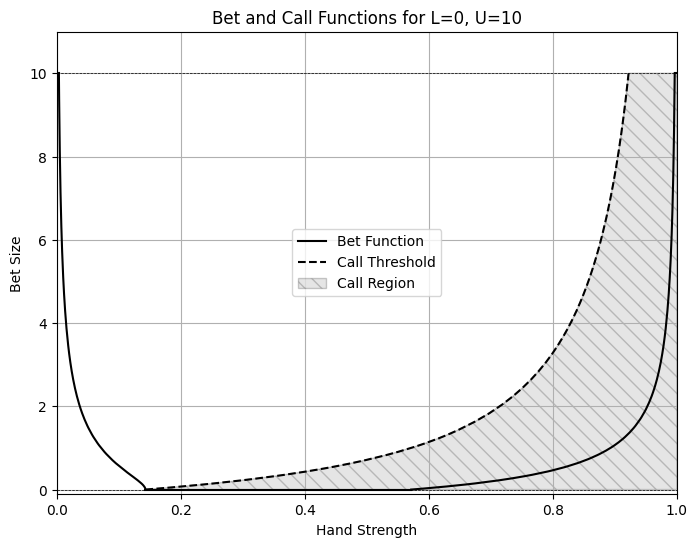
\includegraphics[width=\textwidth]{limit_continuous_0_10.png}
        \end{minipage}
        \hspace{0.05\textwidth}
        \begin{minipage}{0.6\textwidth}
            \centering
            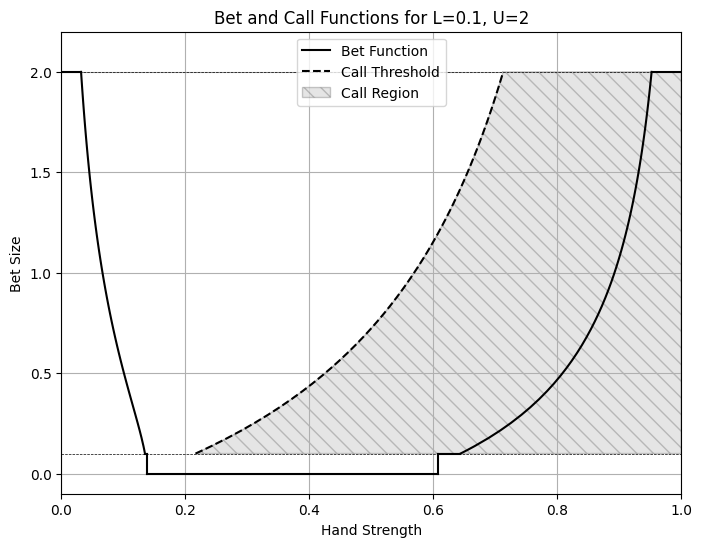
\includegraphics[width=\textwidth]{limit_continuous_0.1_2.png}
        \end{minipage}
        \vspace{0.5cm}\\
        \begin{minipage}{0.6\textwidth}
            \centering
            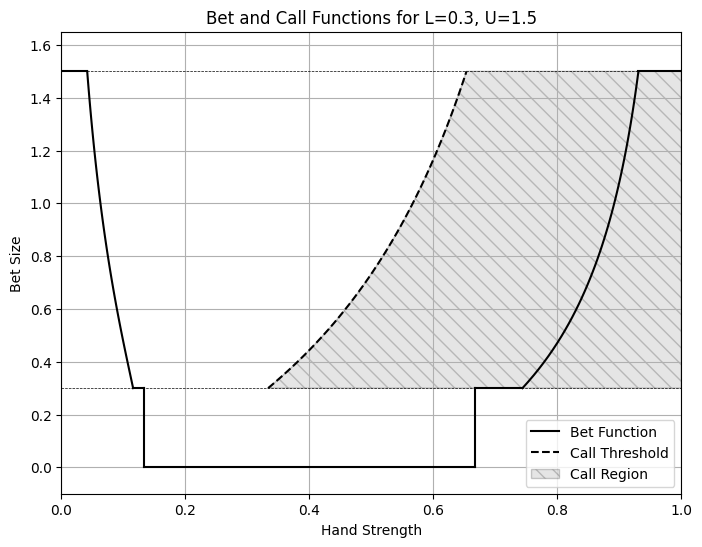
\includegraphics[width=\textwidth]{limit_continuous_0.3_1.5.png}
        \end{minipage}
        \hspace{0.05\textwidth}
        \begin{minipage}{0.6\textwidth}
            \centering
            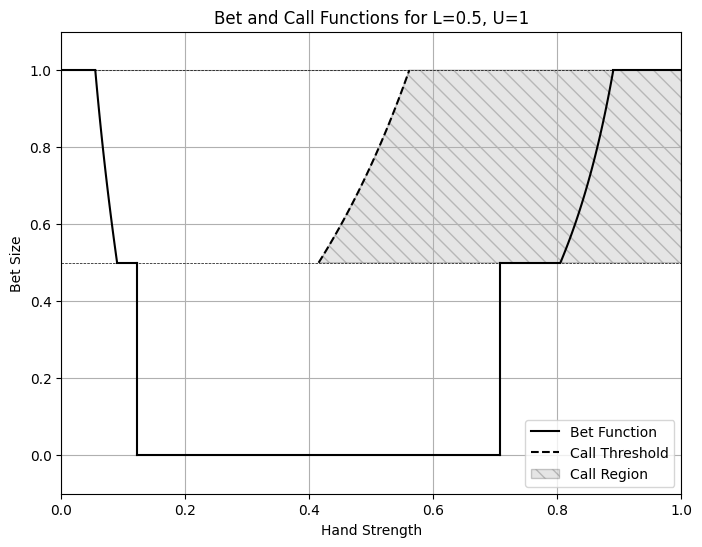
\includegraphics[width=\textwidth]{limit_continuous_0.5_1.png}
        \end{minipage}
    \end{adjustwidth}
    \caption{Nash equilibrium strategy profiles for different values of $L$ and $U$, from very lenient to very restricted bet sizes. The bet function maps hand strengths to bet sizes, while the call function gives the minimum calling hand strength for a given bet size. The shaded regions represent the hand strengths for which the caller should call a given bet size.}
    \label{fig:strategyprofile}
\end{figure}


\subsection{Payoff Analysis}

In Nash Equilibrium, a given hand combination $(x, y)$ uniquely determines the bettor's payoff, since both players play pure strategies. We can better understand the strategy profile by examining payoffs for all hand combinations over the unit square $[0, 1]^2$ (see Figure \ref{fig:payoffs}). For comparison, the first and last plots show the payoffs in Fixed-Bet Continuous Poker with a fixed bet size $B=1$ and No-Limit Continuous Poker, respectively. We will explore the relationship between the three games in more detail in section \ref{sec:strategic_convergence}.

\begin{figure}[h!]
    \begin{adjustwidth}{-1in}{-1in}
        % \vspace{-3cm} % Move the figure up into the top margin
        \centering
        \begin{minipage}{0.4\textwidth}
            \centering
            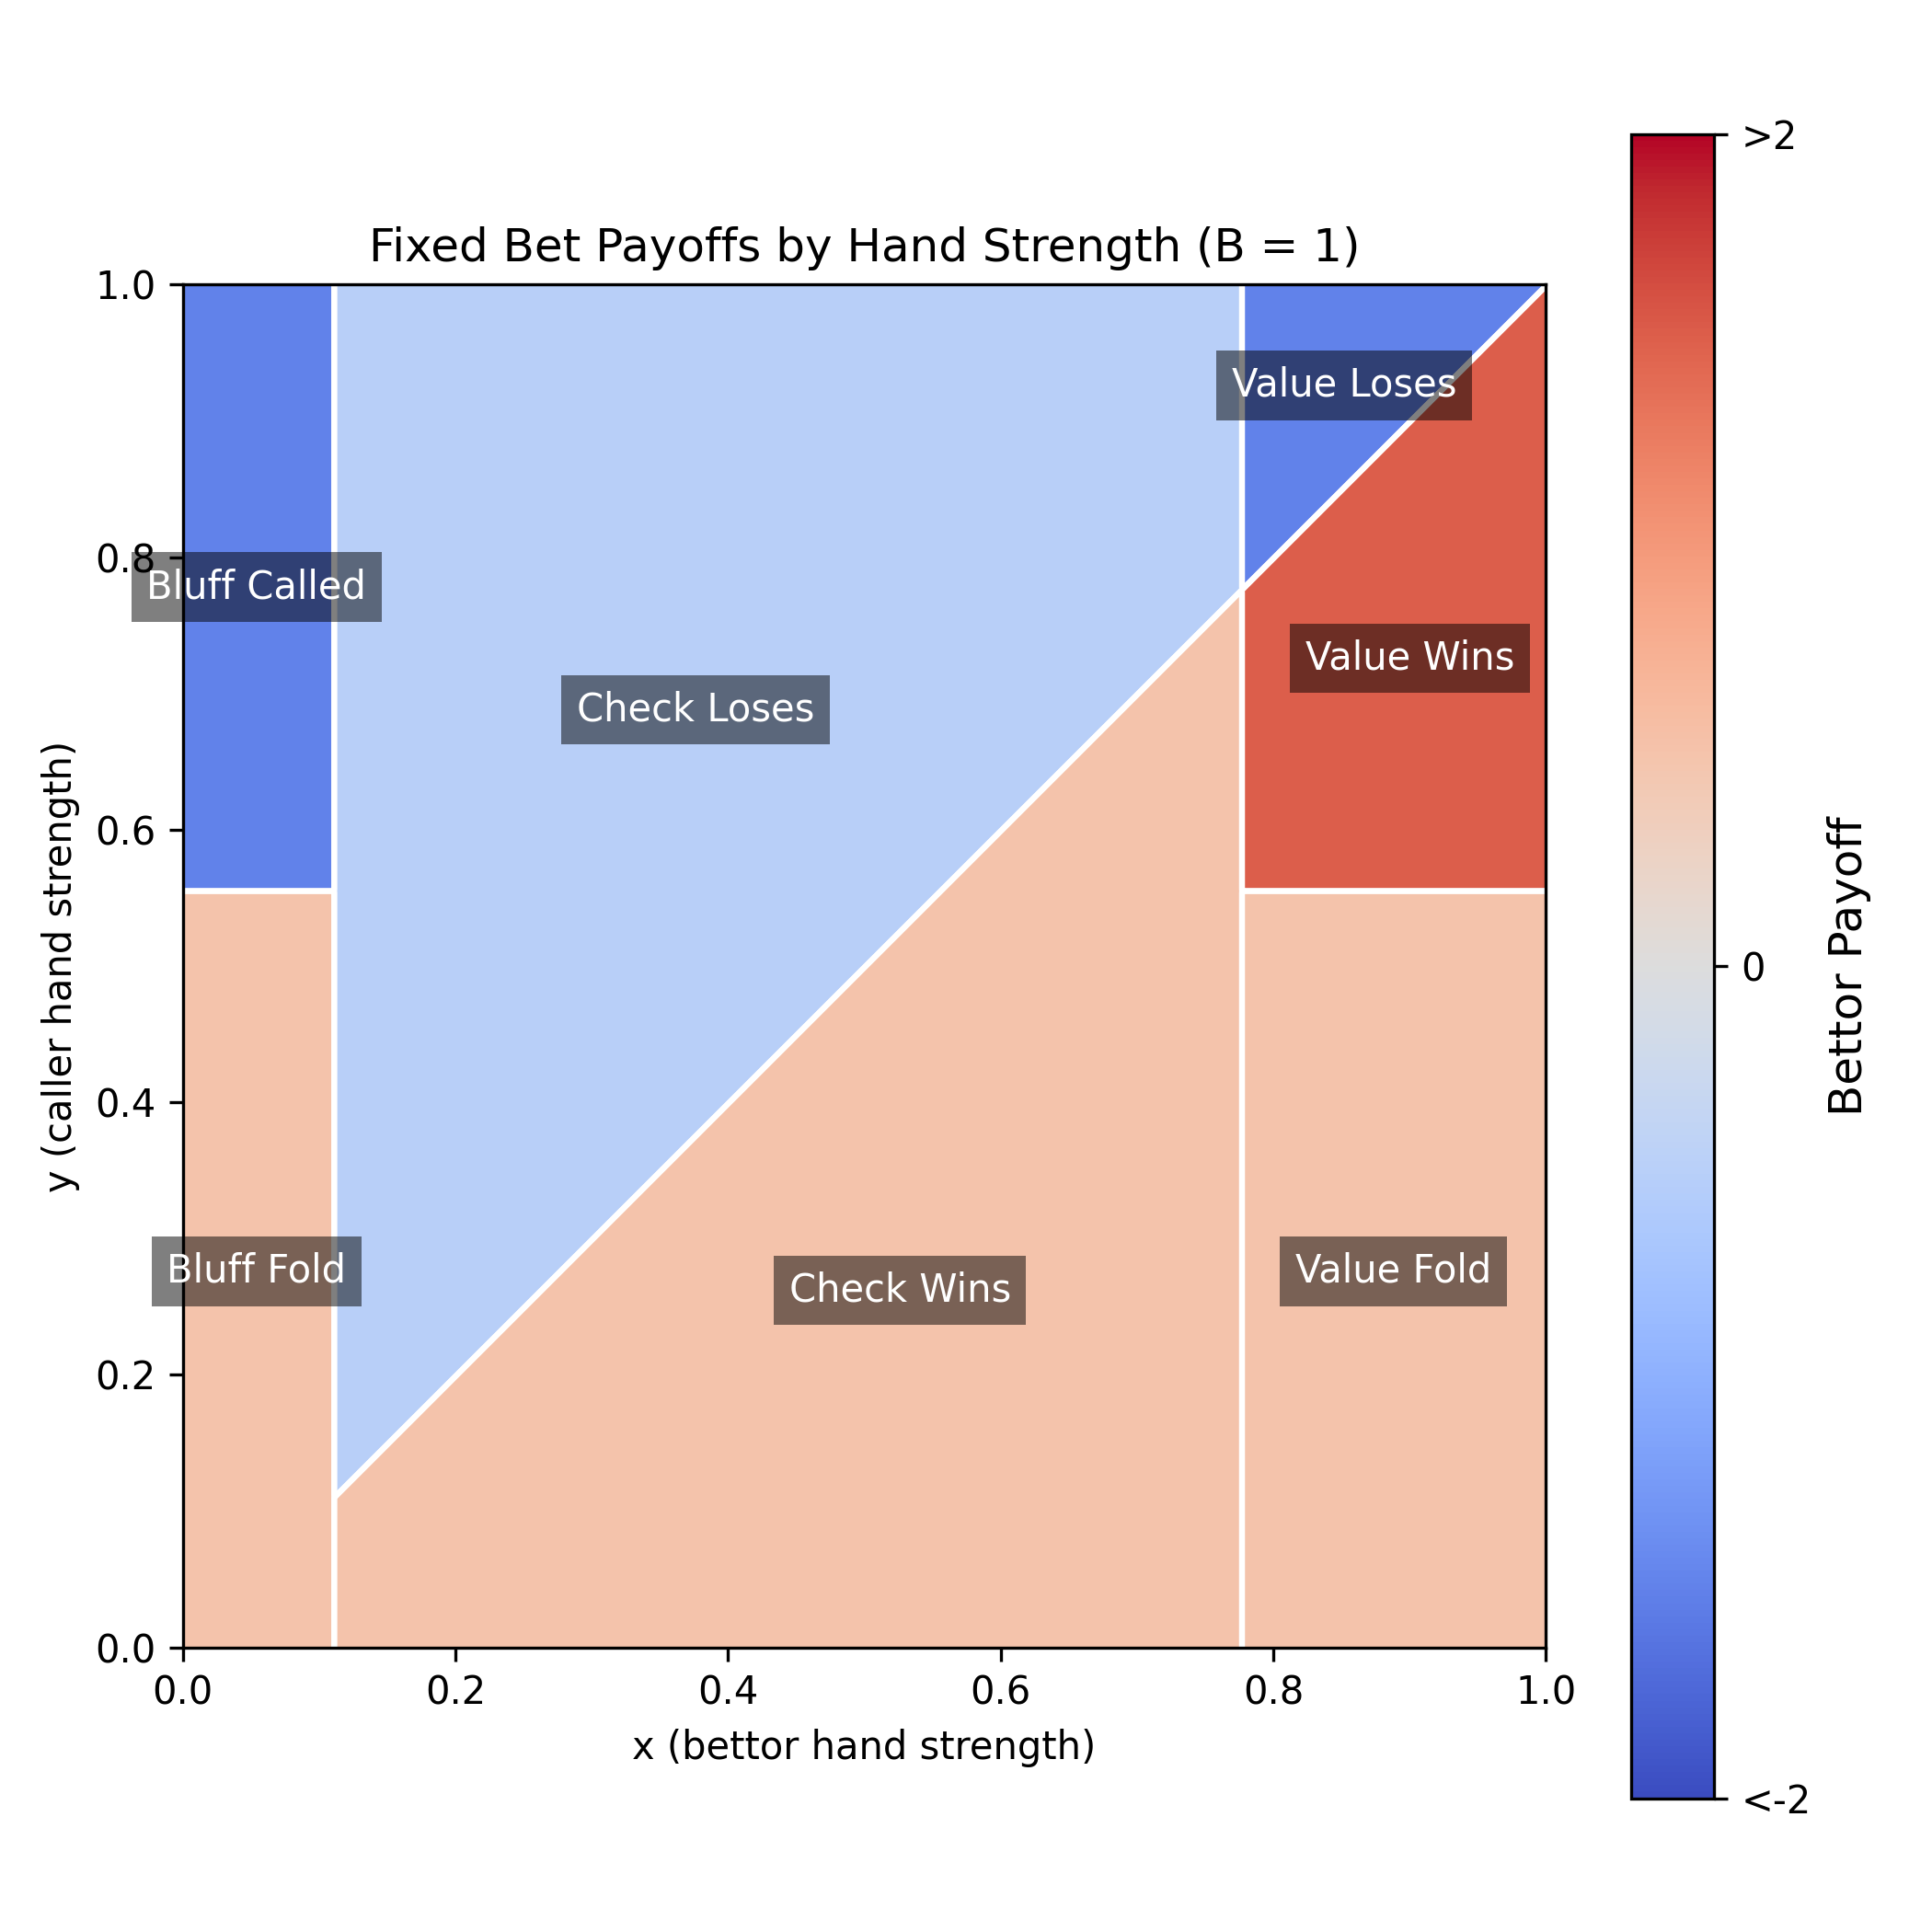
\includegraphics[width=\textwidth]{FixedBet_payoffs.png}
        \end{minipage}
        \hspace{0.02\textwidth}
        \begin{minipage}{0.4\textwidth}
            \centering
            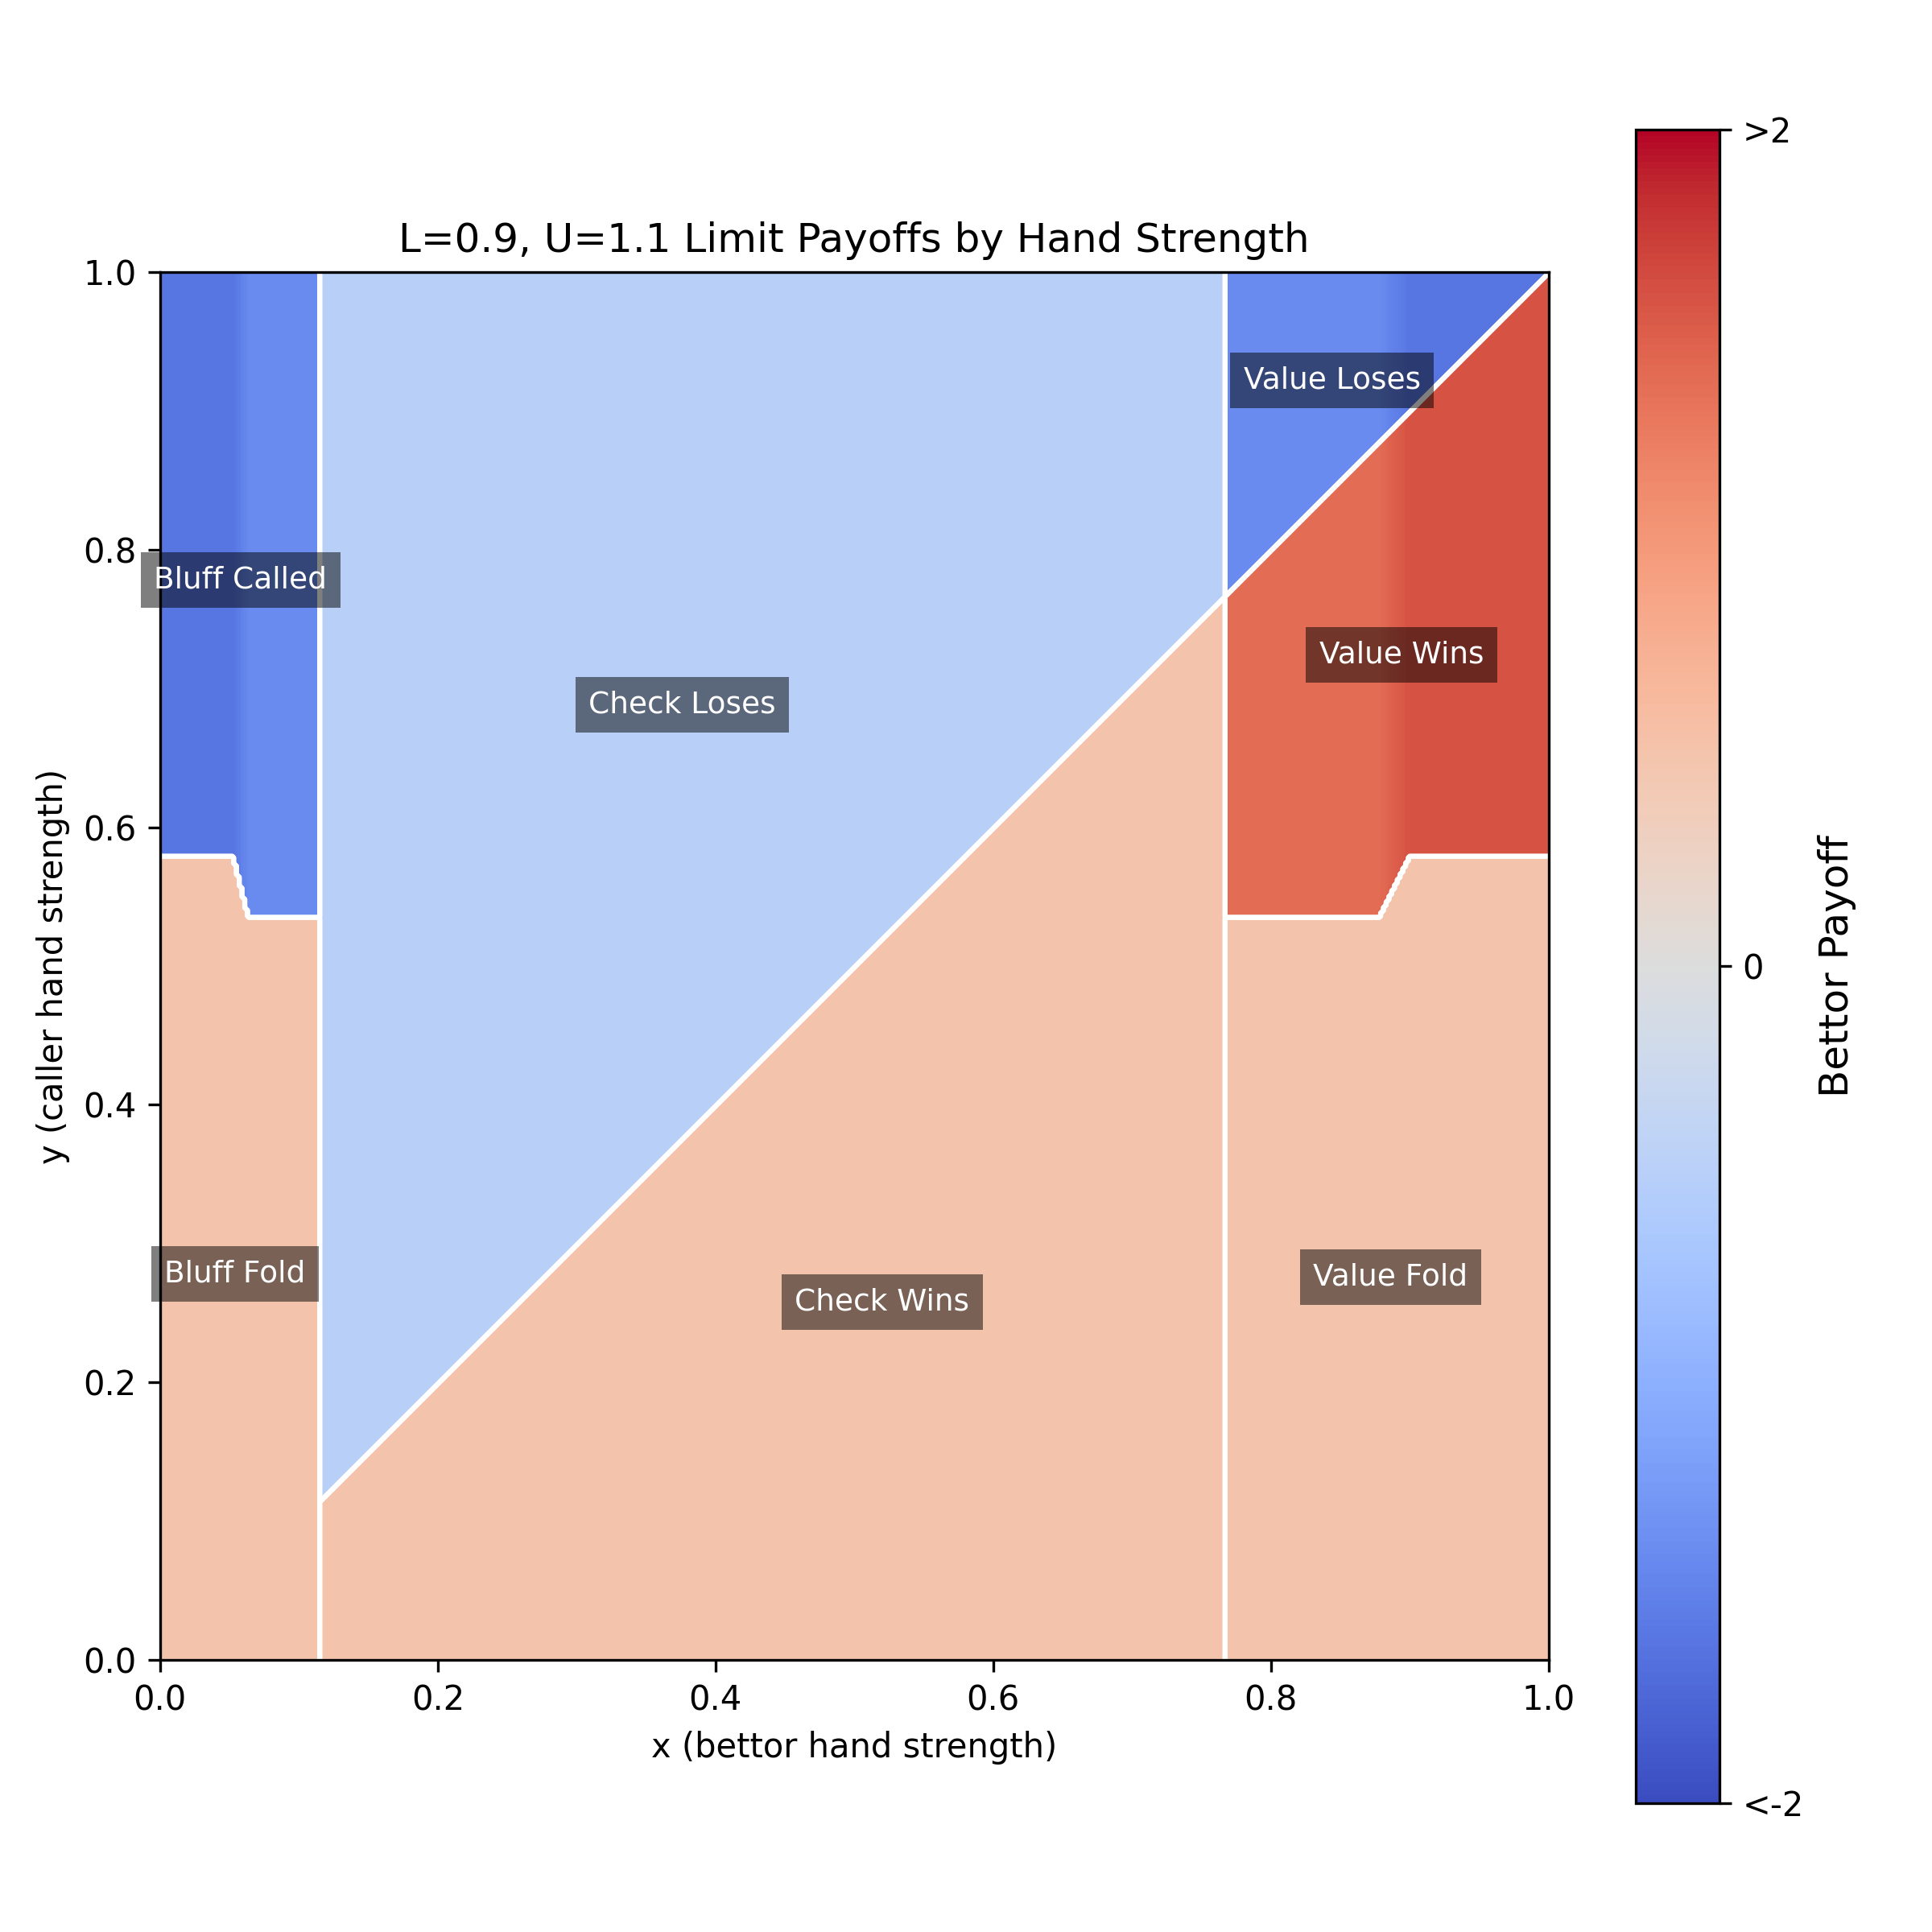
\includegraphics[width=\textwidth]{LU_payoffs_0.9_1.1.png}
        \end{minipage}
        \hspace{0.02\textwidth}
        \begin{minipage}{0.4\textwidth}
            \centering
            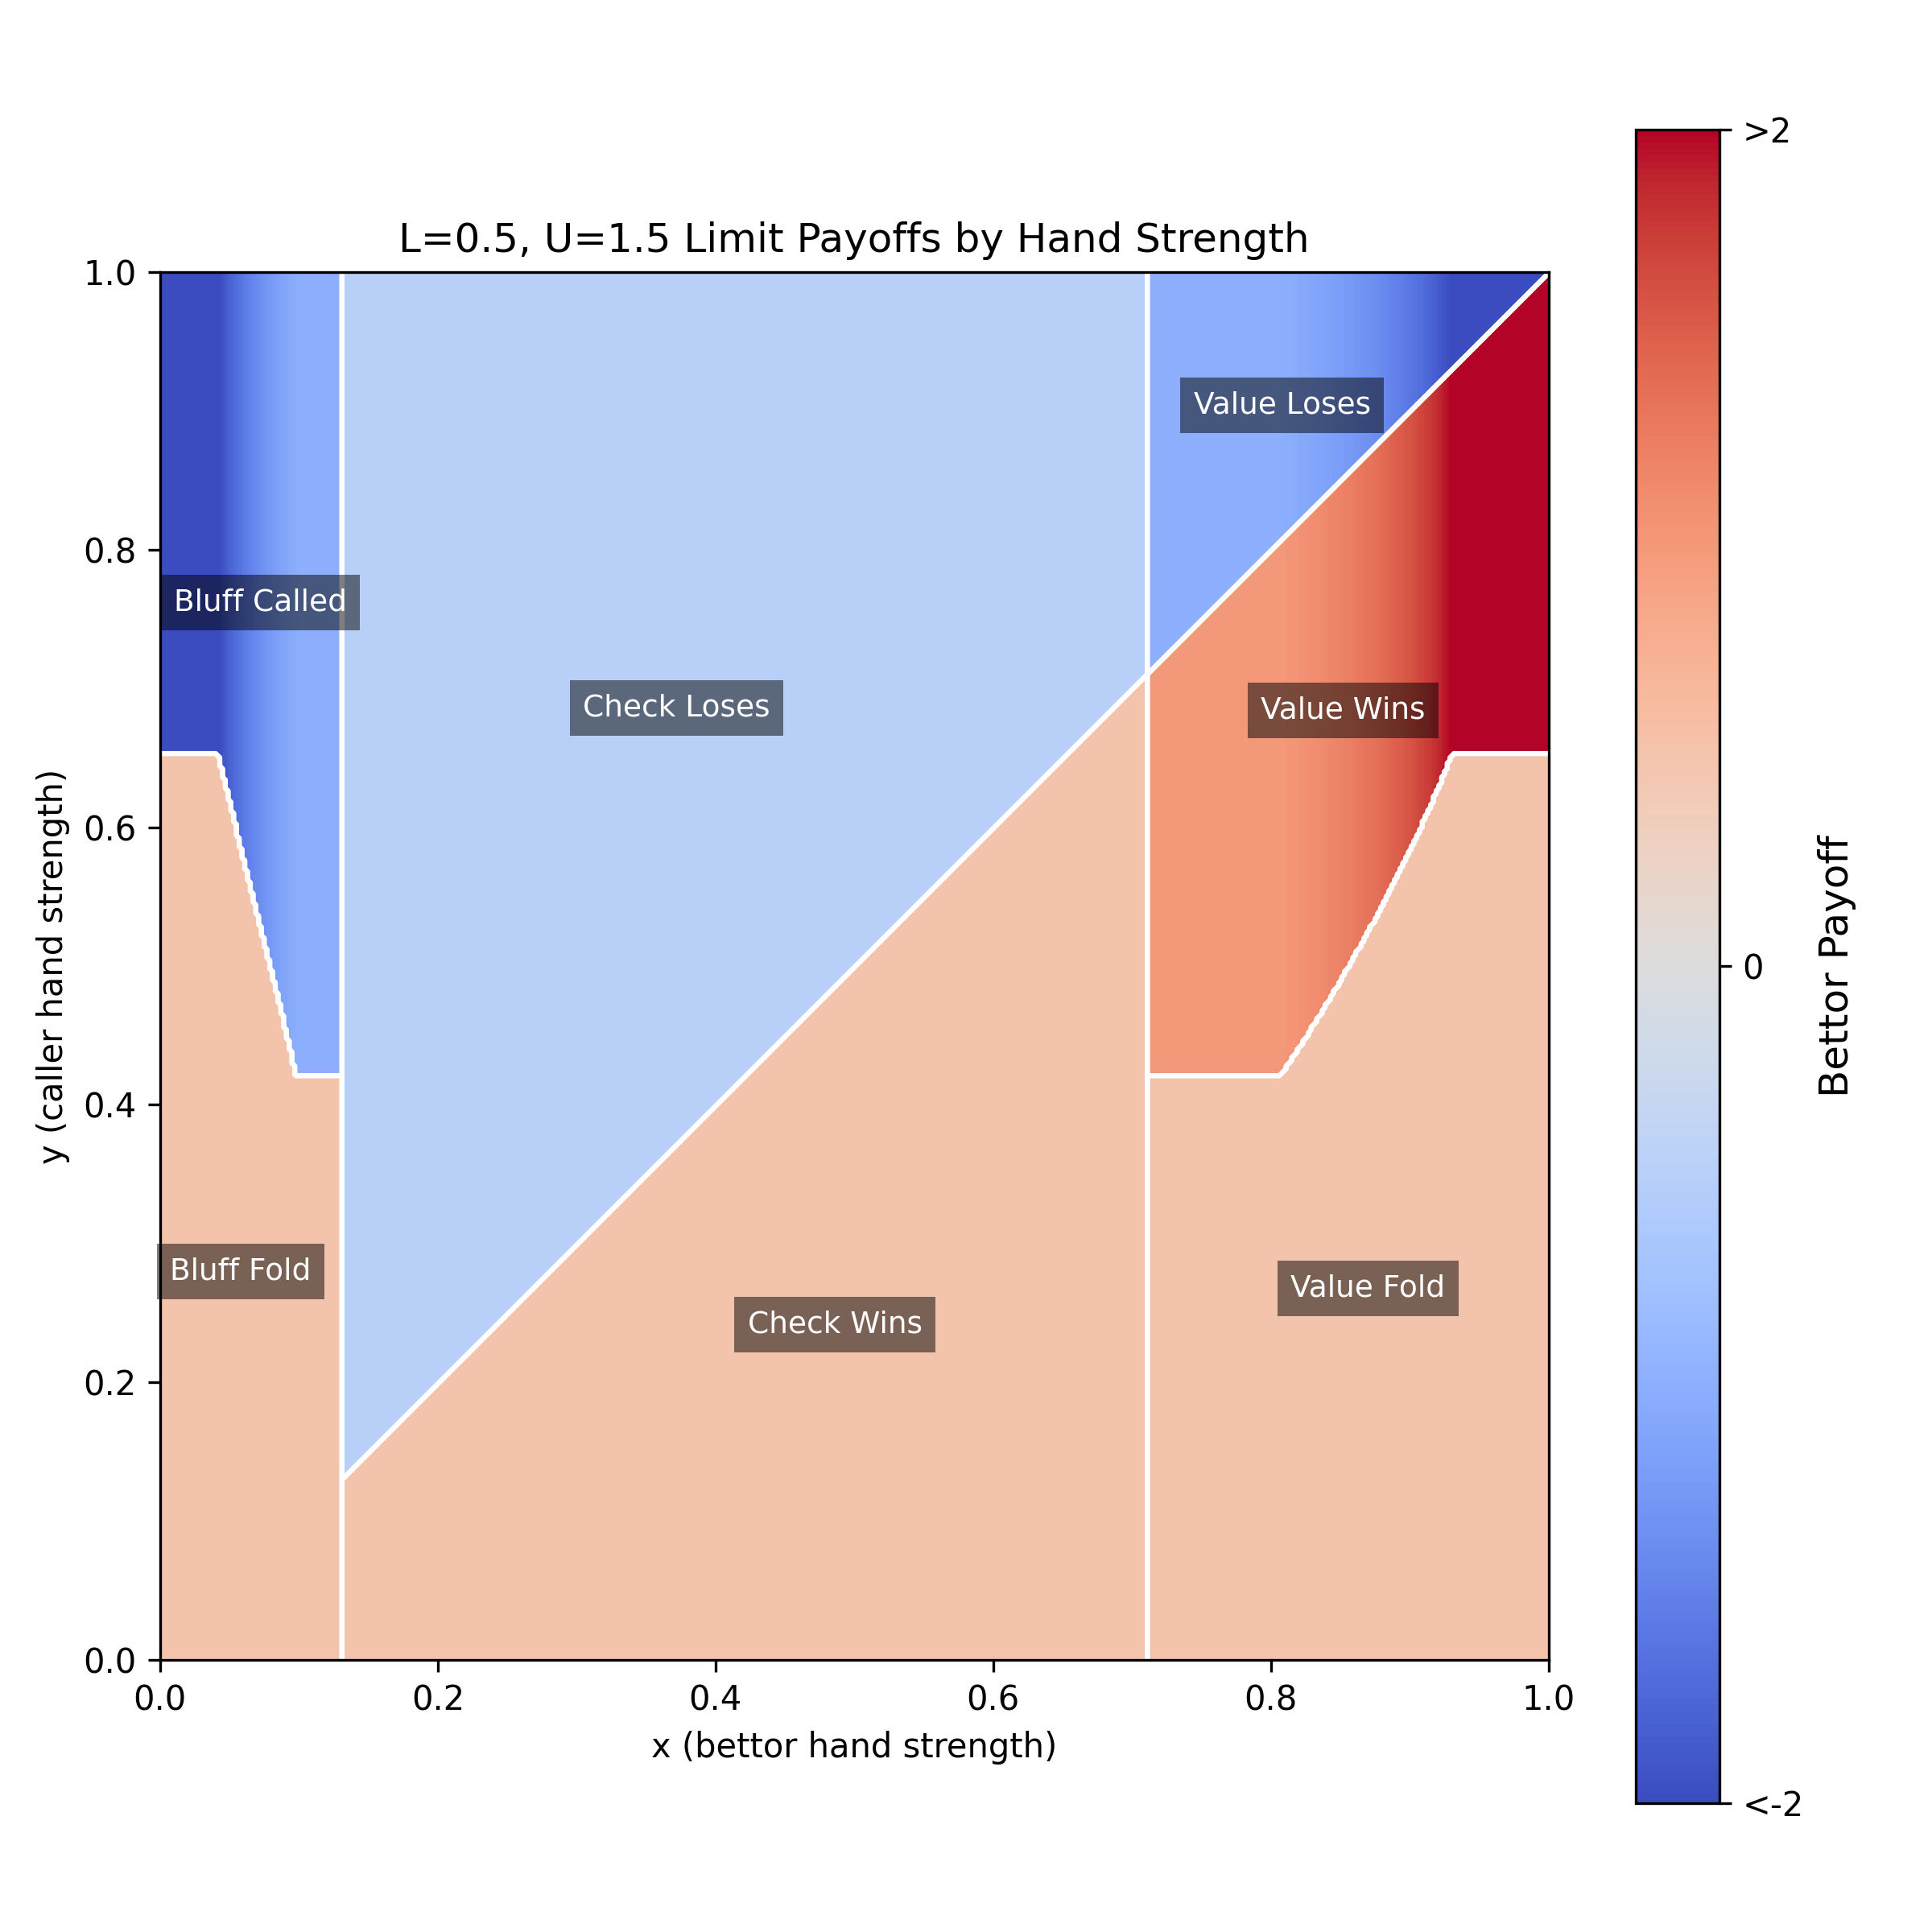
\includegraphics[width=\textwidth]{LU_payoffs_0.5_1.5.png}
        \end{minipage}
        \vspace{-0.5cm}\\ % Reduced vertical space
        \begin{minipage}{0.4\textwidth}
            \centering
            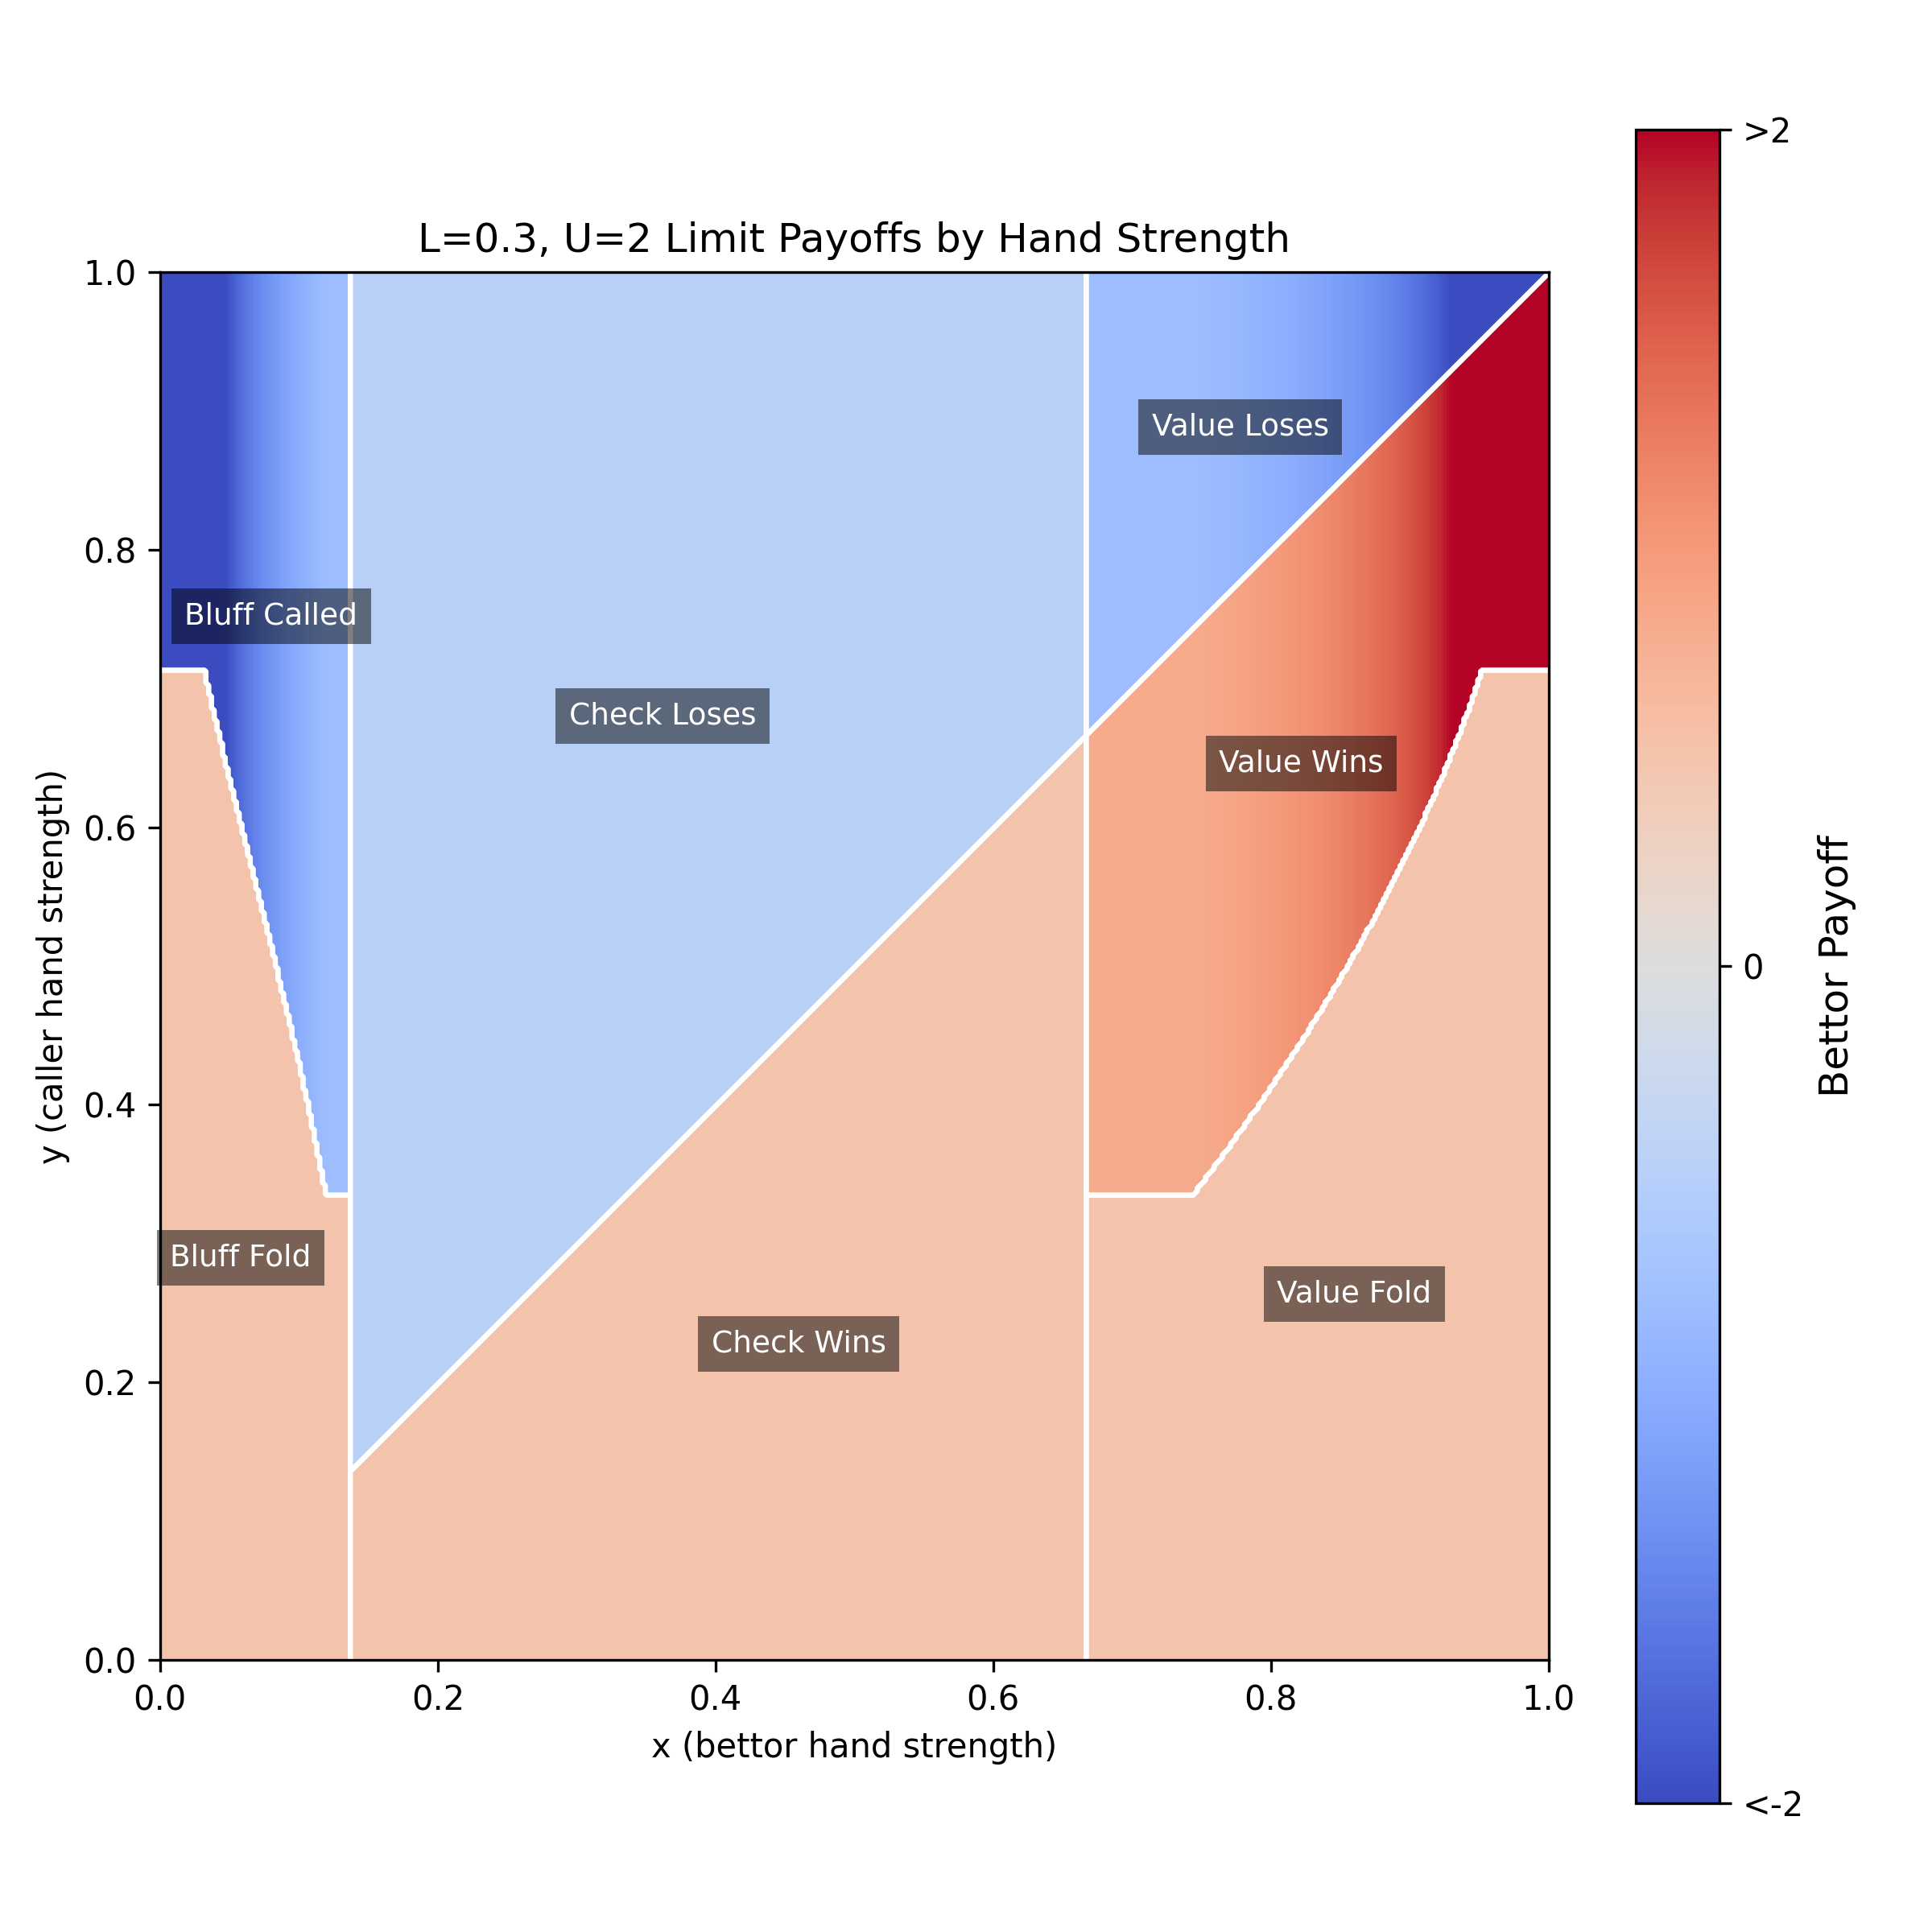
\includegraphics[width=\textwidth]{LU_payoffs_0.3_2.png}
        \end{minipage}
        \hspace{0.02\textwidth}
        \begin{minipage}{0.4\textwidth}
            \centering
            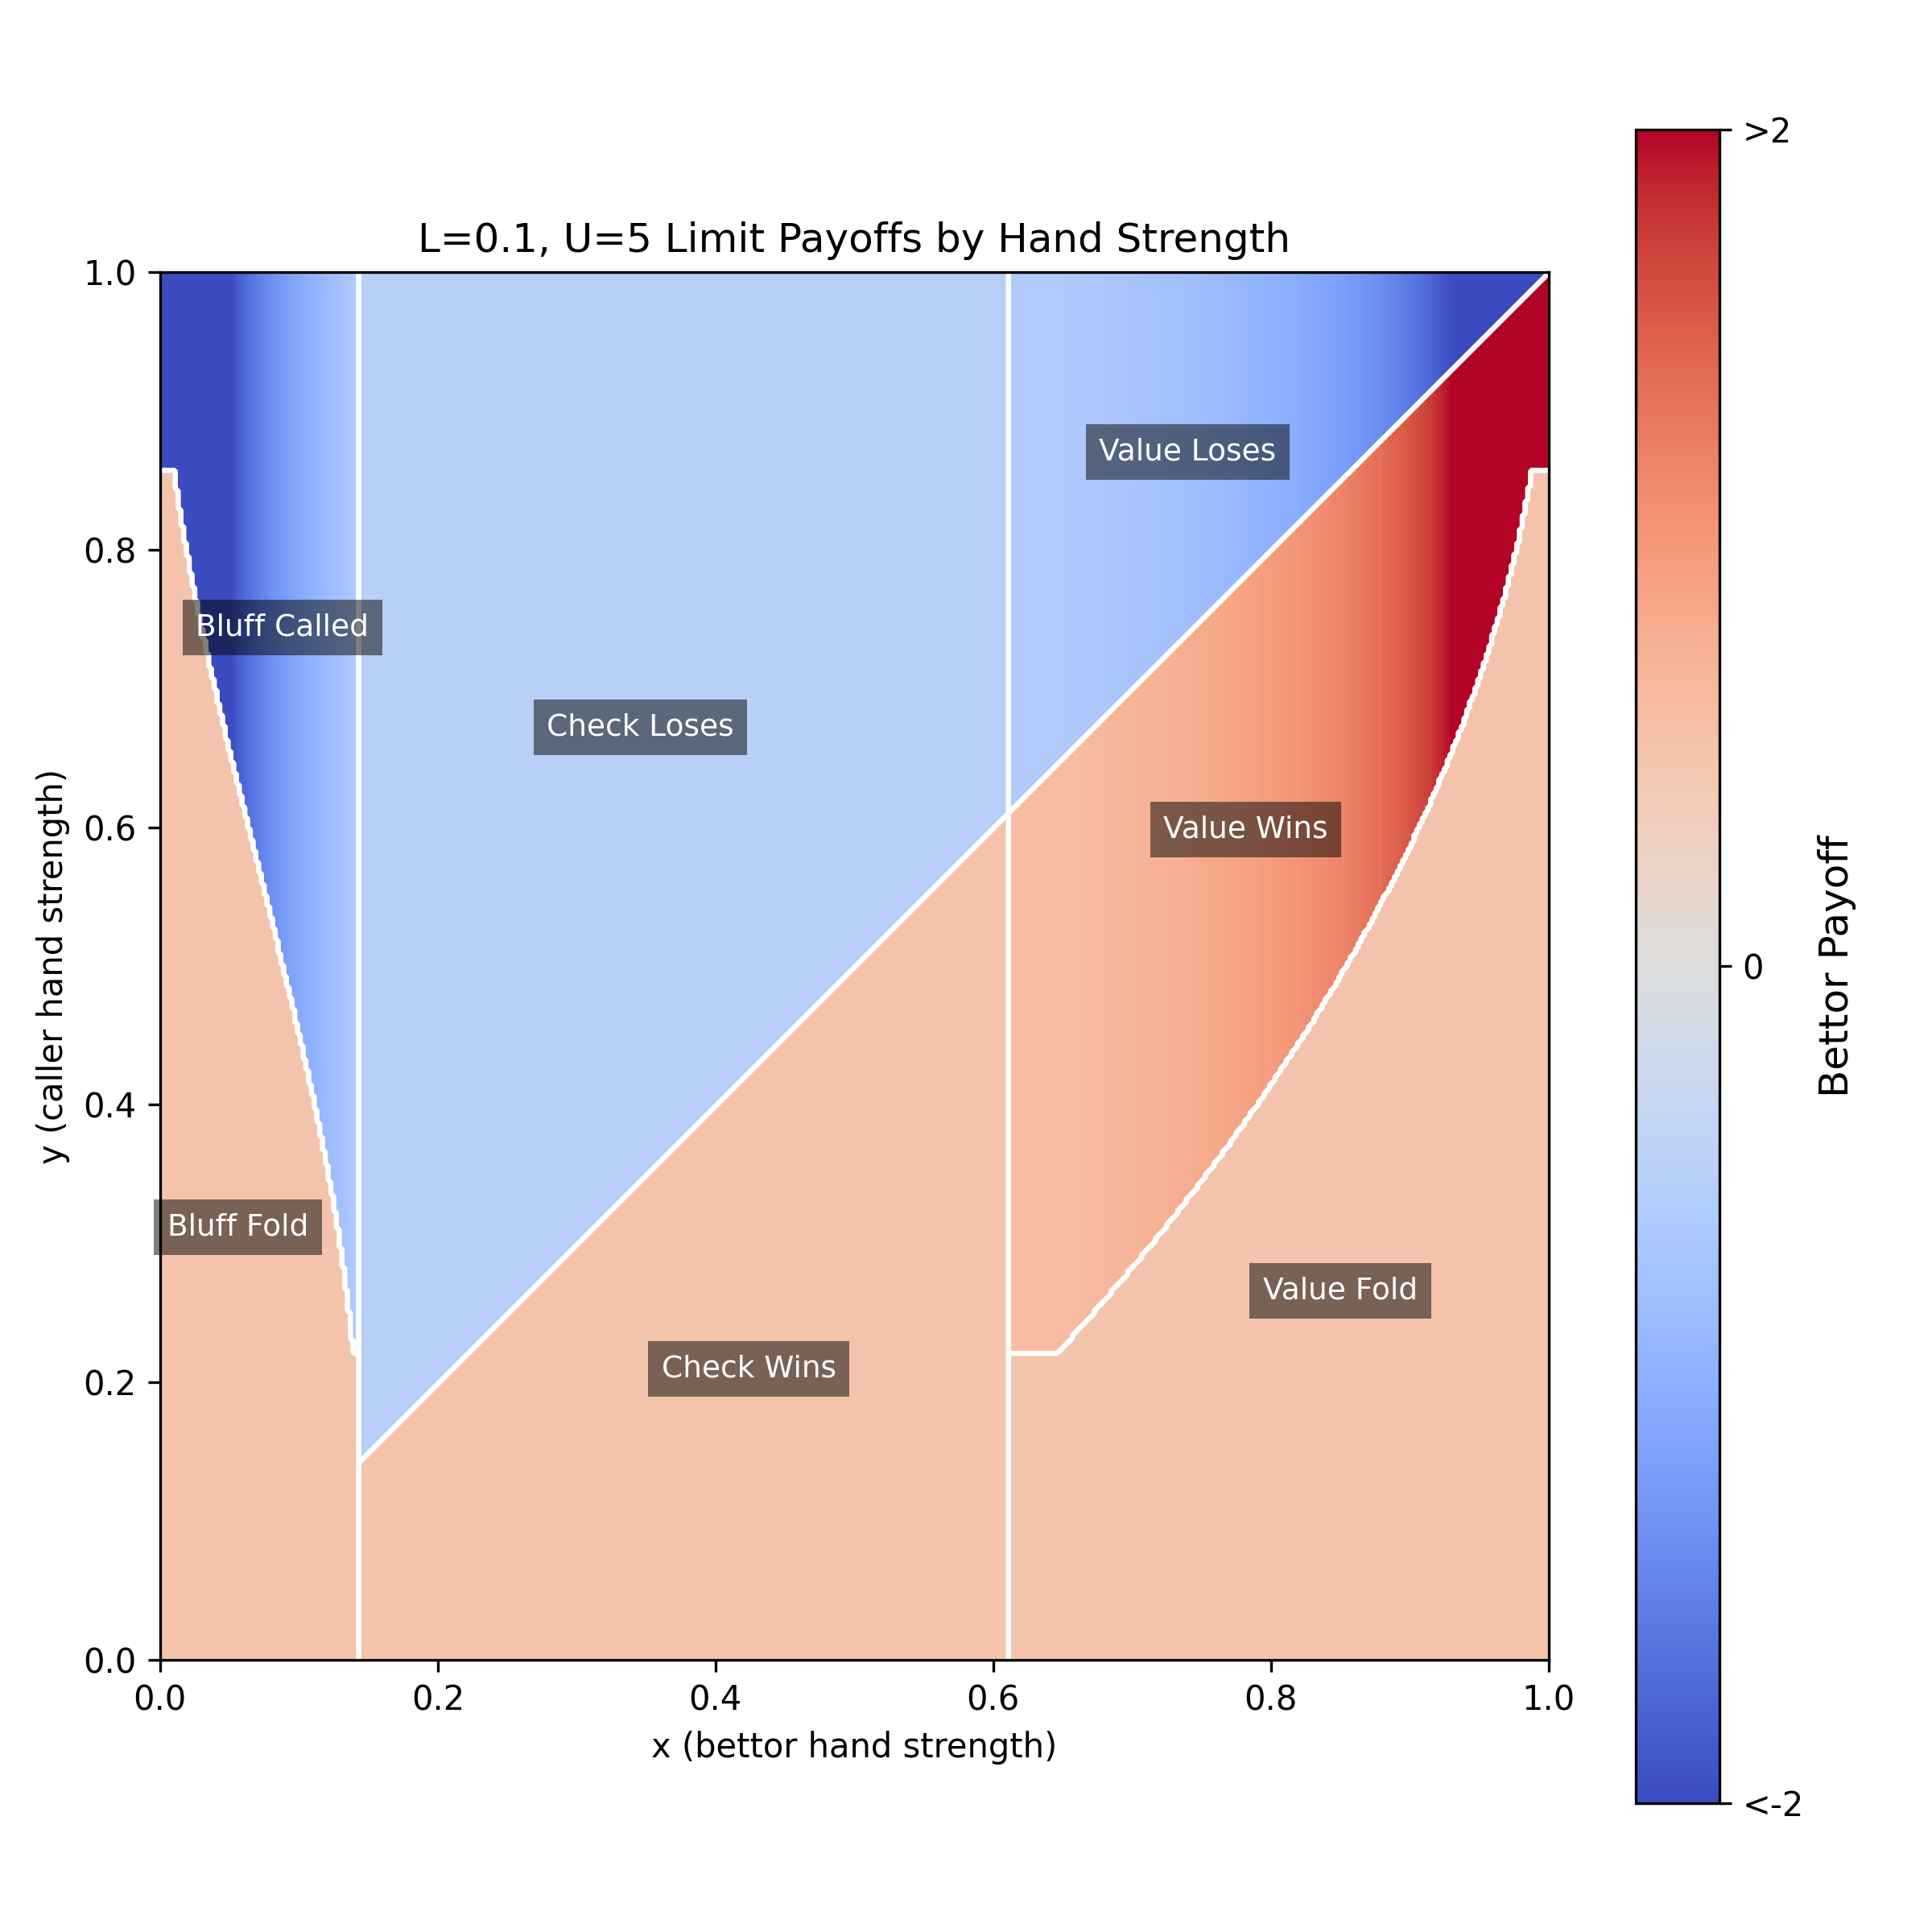
\includegraphics[width=\textwidth]{LU_payoffs_0.1_5.png}
        \end{minipage}
        \hspace{0.02\textwidth}
        \begin{minipage}{0.4\textwidth}
            \centering
            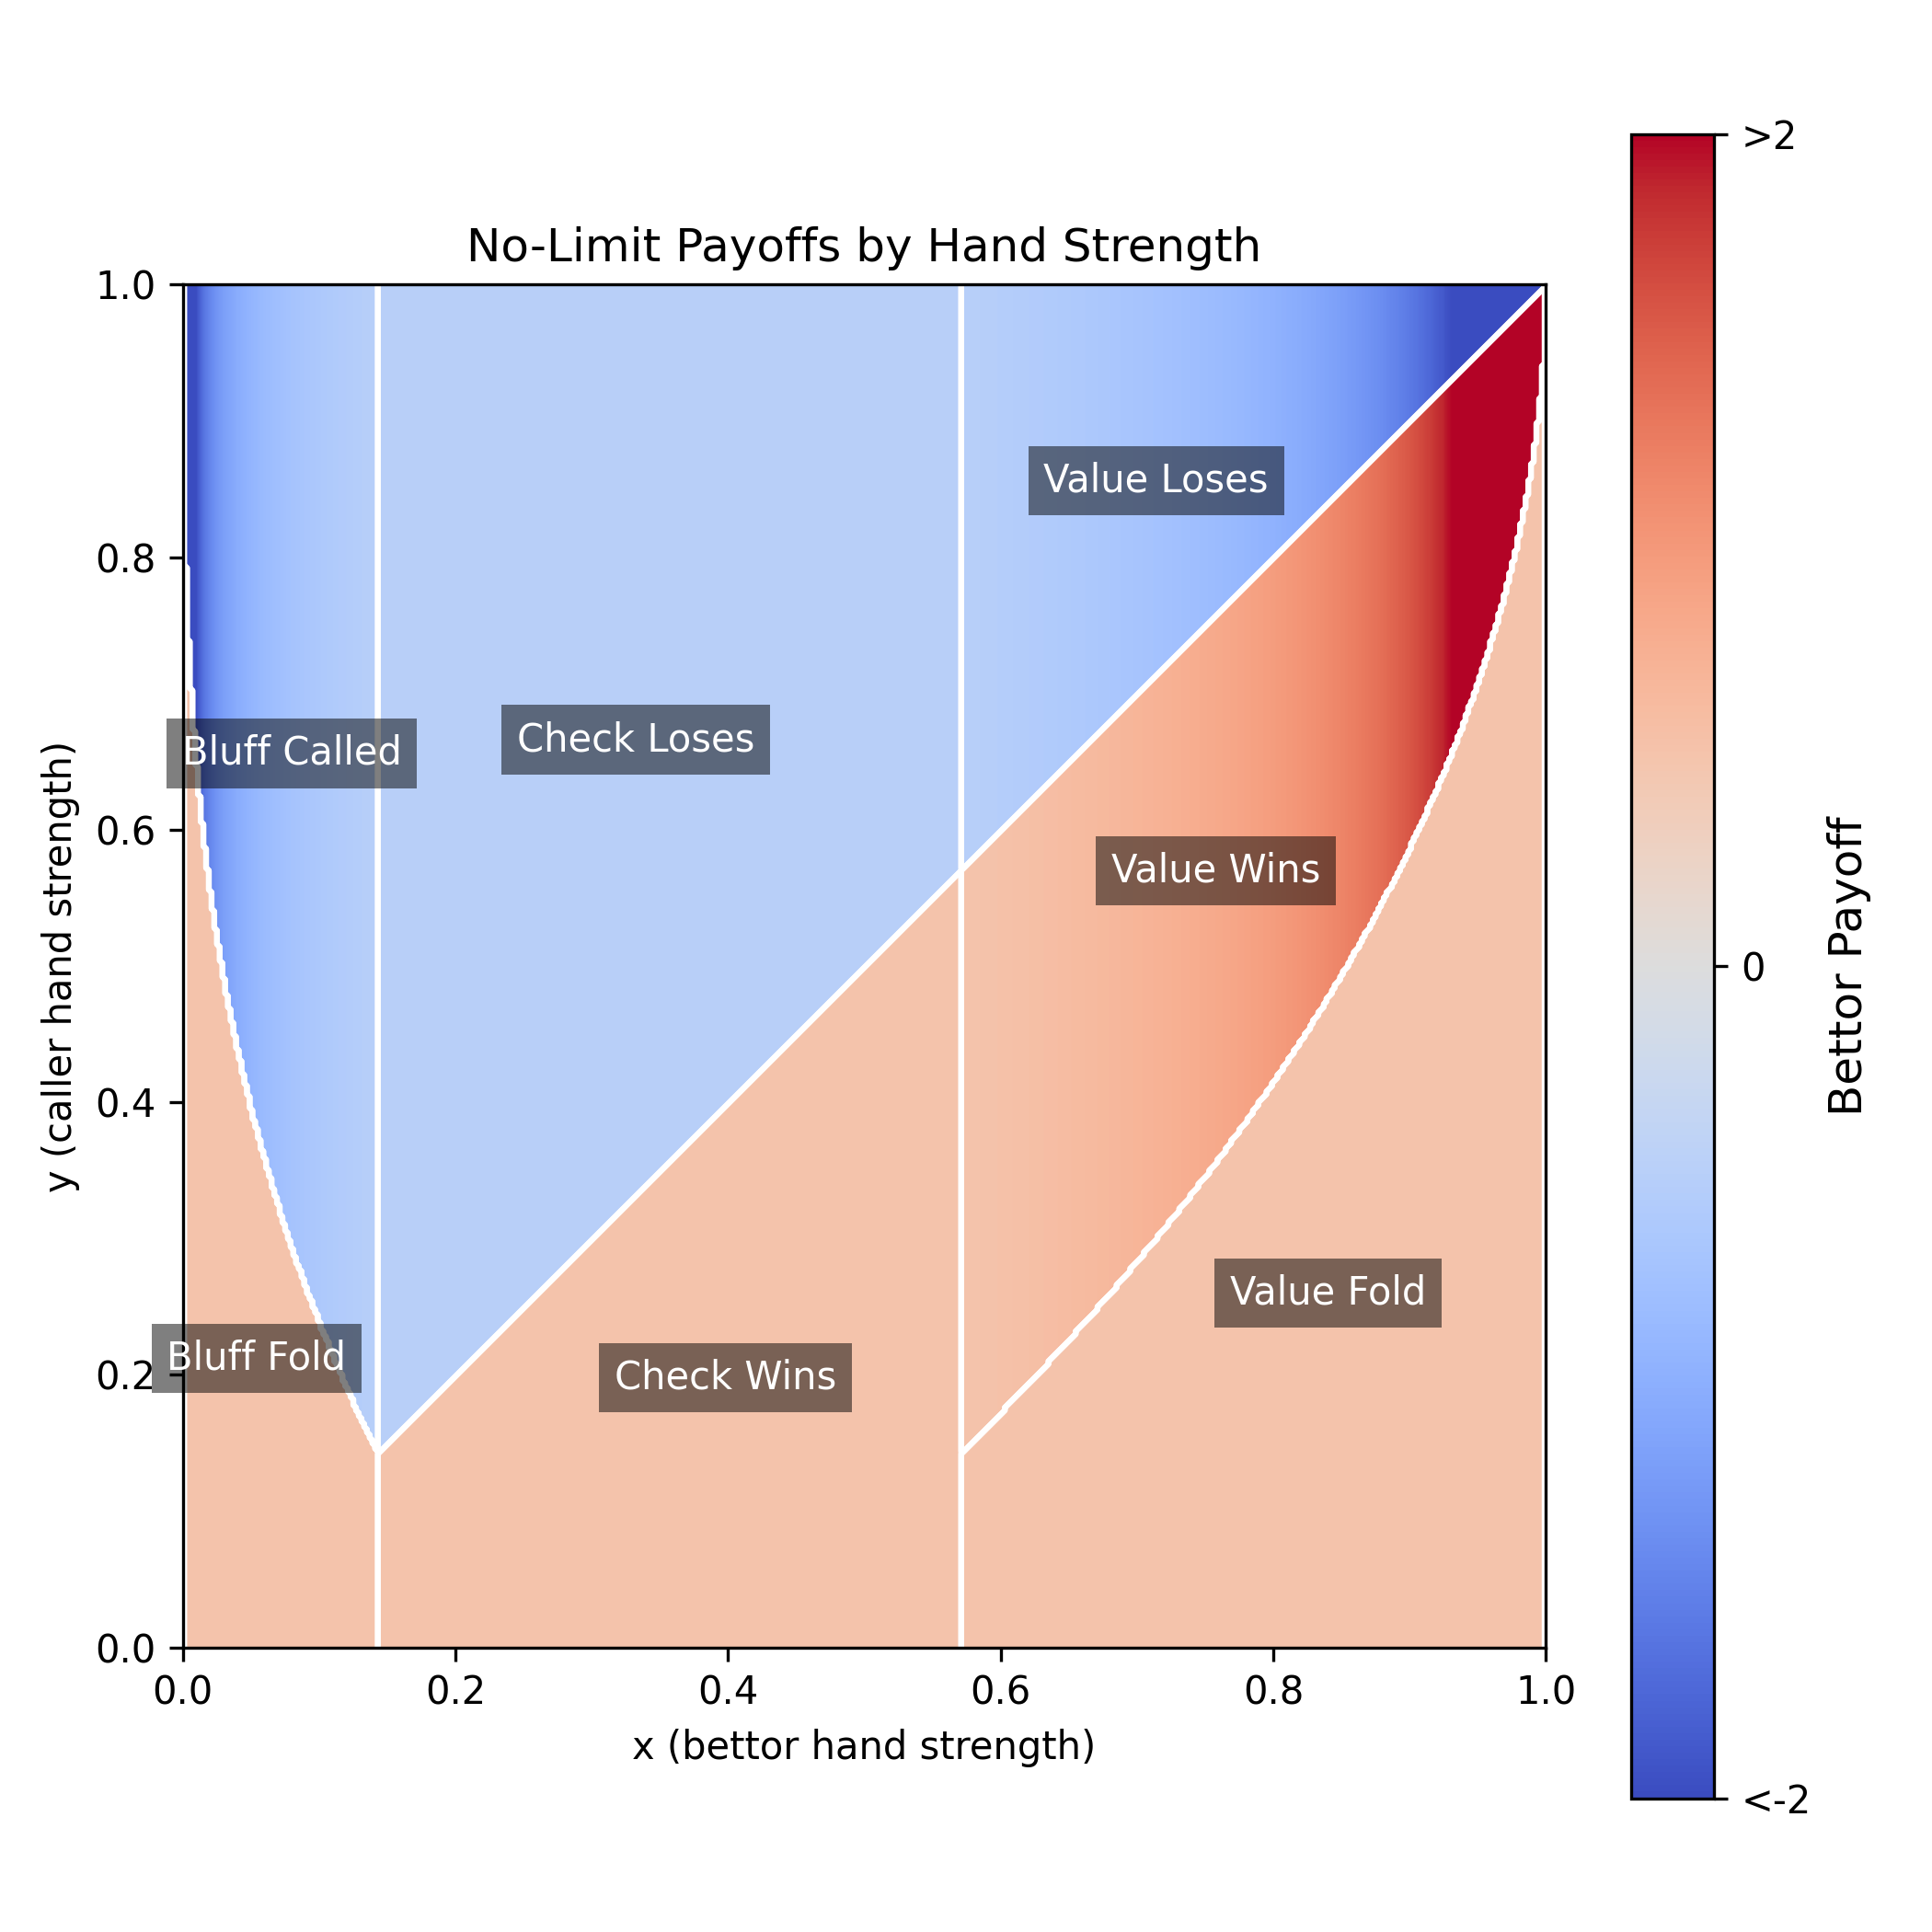
\includegraphics[width=\textwidth]{NoLimit_payoffs.png}
        \end{minipage}
    \end{adjustwidth}
    \caption{Bettor payoffs in Nash equilibrium as a function of hand strengths $x, y$ for fixed bet size $B=1$ (top left), and No-Limit Continuous Poker (bottom right). Intermediate plots show the payoffs for different values of $L$ and $U$ ranging from strict (fixed bet size $B=1$) to lenient (No limits). Regions are labeled according to the outcome of the game in Nash equilibrium.}
    \label{fig:payoffs}
\end{figure}

This visualization gives insight into exactly how the bettor is gaining value from the game. In line with experience of real poker, the biggest wins and losses occur when both hands are strong (top right of any plot), with the stronger of the two hands winning a large pot. However, we also see large payoffs when a very weak bettor bluffs big and gets called by a strong caller (top left). As the limits become more lenient, these cases become more extreme but also less likely, since making and calling maximum bets become more risky for both players. 

\subsection{Expected Value of Bettor's Hand Strengths}

\todo{plots} % EV(x) for different hand strengths}

In addition to considering payoffs for a specific bettor-caller hand combination, we can also consider the expected value of given hand for the bettor, not knowing the hand of the caller. 

% x(2L + 1) - L(c[L] + 1) - 1/2 min value bet
% x(2U + 1) - U(c[U] + 1) - 1/2 max value bet
% x(2vinv[x] + 1) - vinv[x](c[vinv[x]] + 1) - 1/2 intermediate value bet
\begin{theorem}
    \label{thm:ev_bettor}
    \begin{equation}
        EV(x) = \begin{cases}
            x_2-\frac{1}{2} & \text{if } x \leq x_2 \text{ (bluff)} \\
            x-\frac{1}{2} & \text{if } x_2 < x \le x_3 \text{ (check)} \\
            x(2L + 1) - L(c(L) + 1) - \frac{1}{2} & \text{if } x_3 < x < v(L) \text{ (min value bet)} \\
            x(2v^{-1}(x) + 1) - v^{-1}(x)(c(v^{-1}(x)) + 1) - \frac{1}{2} & \text{if } v(L) \leq x \leq v(U) \text{ (intermediate value bet)}\\
            x(2U + 1) - U(c(U) + 1) - \frac{1}{2} & \text{if } x > v(U) \text{ (max value bet)}
        \end{cases}
    \end{equation}
\end{theorem}

\begin{customproof}
    For bluffing hands $x \leq x_2$, we can use a simple argument to show that the hand strength $x$ is actually irrelevant. The bettor never gets called by worse hands, so either the caller folds or calls with the best hand. In either case, the bettor's payoff has no dependence on $x$, so the payoff must be the same for all $x \leq x_2$ (otherwise, a the lower-payoff hands would imitate the strategy of the higher-payoff hands). We know that at $x=x_2$, the bettor is indifferent between bluffing and checking, so the payoff must be $x_2-\frac{1}{2}$ for all $x \leq x_2$.

    For checking hands $x_2 \leq x \leq x_3$, the bettor wins only the ante exactly when they have the best hand, which happens with probability $x$. The value of the ante is $\frac{1}{2}$, so the bettor's expected value is $x-\frac{1}{2}$.

    For any value betting hand, the bettor has three case to consider: the caller folds, the callers calls with a worse hand, or the caller calls with the best hand. We simply sum the expected value of each of these cases.

    \begin{align*}
        EV(x) & = \frac{1}{2} c(s) + (x - c(s)) \left(s+\frac{1}{2}\right) + (1-x) \left(-s-\frac{1}{2}\right)
    \end{align*}
    
    The last three cases come from substituting $L, v^{-1}(x), U$ for $s$ in the expression above and simplifying.
\end{customproof}

We can quickly verify that the bettor's expected value is increasing in $x$. This must be the case, since with any given hand strength, the bettor can always choose to imitate the Nash equilibrium strategy of a weaker hand, so the stronger hand must be at least as good in expectation.

\begin{theorem}
    \label{thm:ev_increasing}
    For any fixed $L, U$, the bettor's expected value $EV(x)$ is increasing in $x$:

    $$ \frac{d}{dx} EV(x) > 0 $$
\end{theorem}

\begin{customproof}
    It is clear from inspection that any checking EV is higher than that of a bluff. We also know that at $x=x_3$, the bettor is indifferent between checking and betting, so the EV of checking and betting must be equal at this point. Therefore, we only need to show that within the checking and value betting regions, the EV is increasing in $x$. This is obvious for checking hands. For value betting hands, we can take the derivative of the expression for $EV(x)$ with respect to $x$ and show that it is always positive. We consider the max and min betting hands first:
    
    \begin{align*}
        \frac{d}{dx} EV(x) & = 2U + 1 > 0 \text{ for } s = U \\
        \frac{d}{dx} EV(x) & = 2L + 1 > 0 \text{ for } s = L
    \end{align*}
    
    For intermediate value betting hands, we can use the chain rule to show that the EV is increasing in $x$:
    
    \begin{align*}
        \frac{d}{dx} EV(x) & = \frac{\partial EV(x)}{\partial x} + \frac{dEV(x)}{ds} \frac{d s}{d x} \\
    \end{align*}

    From the value optimality condition, we know that $\frac{dEV(x)}{ds} = 0$ (otherwise, the bettor could gain value by varying the bet size). Clearly, $\frac{\partial EV(x)}{\partial x} > 0$.  Therefore, the derivative is positive, and the EV is increasing in $x$ for all value betting hands.
\end{customproof}

It is worth noting that the bettors strongest hands (right edge) actually seem to become less likely to make any profit more than the ante as limits increase. These strongest hands make very large bets, which force all but the strongest hands to fold, but win huge pots when they do get called. In more complicated poker variants, it is common to `slowplay' strong hands by checking or making small bets to induce bluffs from the opponent. In LCP, there is only one betting round and the caller is not allowed to raise, both of which make slowplaying obsolete. With extremely strong hands, the benefit of winning a large pot when betting big outweighs the lower likelihood of getting called.

\subsection{Effect of Increasing $U$}

\subsubsection{Expected Payoff of Value-Betting Hands}

It may seem unsurprising that strong hangs become less likely to get called as limits increase, but what about the actual expected payoff of these hands? Does the expected value of each hand continue increasing as we increase $U$? The answer is no. In fact, for any fixed hand strength $x$, the expected payoff of that hand decreases in $U$ if $x$ makes any bet other than the maximum (and even then, unless $x$ is sufficiently high). Increasing $U$ only gives the bettor more options, so how is it possible that the expected payoff of a wide range of their hands decreases? And which hands are gaining expected payoff to offset this? This is a surprising result, and it is worth exploring in more detail.

\begin{theorem}
    \label{thm:payoff_increasing}
    For any fixed value-betting hand strength $x>1/2$, in Nash equilibrium, the expected payoff $EV(x)$ is increasing in $U$ if  and decreasing in $U$ otherwise.

    \begin{align*}
        \frac{d}{dU} EV(x) > 0 & \text{ if } x > v(U) \\ 
        \frac{d}{dU} EV(x) < 0 & \text{ if } x_3 < x < v(U) 
    \end{align*}
\end{theorem}

Before proving the theorem, we will walk through some lemmas which explore how all the relevant variables change as we increase $U$, including the bluffing threshold $x_2$, the bet size $v^{-1}(x)$, and the calling cutoff $c(s)$.

\subsubsection{Bluffing Threshold}

We begin by showing that $x_2$, the boundary hand strength between bluffing and checking, is increasing in $U$. This means that for fixed $L$, increasing the upper limit $U$ makes the bettor bluff with more hands. 

\begin{lemma}
    \label{lem:x2_increasing}
    For any fixed $L \in [0, U]$,
    $$ \frac{\partial x_2}{\partial U} > 0 $$
\end{lemma}

\begin{customproof}
    Taking the partial derivative of $x_2$ with respect to $U$ in Mathematica and rearranging terms gives:
    
    $$\frac{\partial x_2}{\partial U} = \frac{18 (L+1)^6 (U+1)^2}{\left(A_1 + L^3 A_2 + 3 L^2 A_1 + 3 L A_1 \right)^2}$$

    Which is always positive since $L \in [0, U]$, $U \in [0, \infty)$, and $A_1, A_2$ are both positive-coefficient polynomials in $L$ and $U$.   
\end{customproof}

\subsubsection{Bet Size}

We now show that if we fix $x$ at any intermediate value-betting hand strength (betting neither the minimum nor maximum bet size) and then increase $U$, the bet size $s$ made by $x$ decreases. The intermediate value-betting hands are exactly $x \in [x_3, v(U)]$ and their bet sizes are given by $s = v^{-1}(x)$, so we get the following lemma:

\begin{lemma}
    \label{lem:v_inverse_decreasing}
    For any fixed $x \in [x_3, v(U)]$, 
    \[ 
        \frac{d}{dU} v^{-1}(x) < 0
    \]
\end{lemma}

\begin{customproof}
    Recall that 
    $$v^{-1}(x) = -\frac{\sqrt{(4 x-4) (2 x_2-2)}}{4 x-4}-1$$
    Where $x_2$ is a function of $L$ and $U$. Importantly, $v^{-1}(x)$ is only dependent on $U$ through $x_2$, so we can use the chain rule to take the derivative with respect to $U$:
    \begin{align*}
        \frac{d}{dU} v^{-1}(x) & = \frac{\partial v^{-1}(x)}{\partial x_2} \frac{\partial x_2}{\partial U}
    \end{align*}

    The first term is 

\begin{align*}
    \frac{\partial v^{-1}(x)}{\partial x_2} & = - \frac{1}{\sqrt{(4 x-4) (2 x_2-2)}} \\
    &= - \frac{1}{(v^{-1}(x)+1)(4-4x)}
\end{align*}

    Which is always negative since $x \in [0, 1]$ and $v^{-1}(x) >0 $. We know that the second term is positive by Lemma \ref{lem:x2_increasing}.

    Therefore, the product of the two terms is always negative, so the bet size of intermediate bets is decreasing in $U$.
\end{customproof}

\subsubsection{Calling Cutoff}

We now turn our attention to how the calling cutoff $c(s)$ varies with $U$. Recall that $c(s)$ is defined as the minimum hand strength $y$ which should call a bet of size $s$ and is given in Nash equilibrium by:

$$c(s) = \frac{x_2 + s}{s+1}$$

We are specifically interested in how $c(v^{-1}(x))$ varies with $U$ for $x \in [x_3, v(U)]$, since this represents how the calling cutoff changes both directly from a strategic change, as well as indirectly due to the lower bet size $s$. It turns out that the calling cutoff is increasing in $U$ for all $x \in [x_3, v(U)]$. This is surprising because we just showed that the bet size $s$ is decreasing in $U$, and we expect smaller bets to be called more often. For reasons we will see later, this effect is overpowered by a strategic shift for the caller, who calls less often for all bet sizes as $U$ increases. 

\begin{lemma}
    \label{lem:c_increasing}
    For any fixed $x \in [x_3, v(U)]$, 
    \[ 
        \frac{d}{dU} c(v^{-1}(x)) > 0
    \]
\end{lemma}

\begin{customproof}
    As mentioned above, $c(s)$ is dependent on $U$ in two distinct ways -  directly through $x_2$, which can be interpreted as the caller changing strategy as the game changes - but also indirectly in response to how the bet size $s = v^{-1}(x)$ is dependent on $U$. We use the multivariate chain rule to express $\frac{d}{dU} c(v^{-1}(x))$ in terms of these two dependencies:
    \begin{align*}
        \frac{d}{dU} c(v^{-1}(x)) & = \frac{\partial c(s)}{\partial s} \frac{d v^{-1}(x)}{d U} + \frac{\partial c(s)}{\partial x_2} \frac{\partial x_2}{\partial U}
    \end{align*}
    
    The two partial derivatives of $c(s)$ are:

    $$ \frac{\partial c(s)}{\partial s} = \frac{1-x_2}{(s+1)^2} \; \; \; \text{and} \; \; \; \frac{\partial c(s)}{\partial x_2} = \frac{1}{s+1} $$

    Substituting $s = v^{-1}(x)$, we can further simplify the first term:

    \begin{align*}
        \frac{\partial c(s)}{\partial s} \bigg|_{s=v^{-1}(x)} & = \frac{1-x_2}{(v^{-1}(x)+1)^2} \\
        & = 2-2x
    \end{align*}

    And as we showed in the proof of Lemma \ref{lem:x2_increasing}, $\frac{d v^{-1}(x)}{d U}$ is given by:

    $$ \frac{d v^{-1}(x)}{d U} = \frac{-1}{(v^{-1}(x)+1)(4-4x)} \frac{\partial x_2}{\partial U} $$

    Substituting all of these with $s = v^{-1}(x)$:

    \begin{align*}
        \frac{d}{dU} c(v^{-1}(x)) & = 
        \left(2-2x\right) 
        \left(\frac{-1}{(v^{-1}(x)+1)(4-4x)}\right) 
        \left(\frac{\partial x_2}{\partial U}\right) 
        + \left(\frac{1}{v^{-1}(x)+1}\right) 
        \left(\frac{\partial x_2}{\partial U}\right)\\
        & = \left( \frac{1}{v^{-1}(x)+1} \right) 
        \left( \frac{\partial x_2}{\partial U} \right)
        \left( -\frac{2-2x}{4-4x} + 1\right) \\
        & = \left( \frac{1}{v^{-1}(x)+1} \right) 
        \left( \frac{\partial x_2}{\partial U} \right)
        \left( \frac{1}{2} \right) \\
    \end{align*}

    The first term is positive since $v^{-1}(x) > 0$ and the second term is positive by Lemma \ref{lem:x2_increasing}. Therefore, the product of the two terms is positive, so the calling cutoff is increasing in $U$ for all $x \in [x_3, v(U)]$.

\end{customproof}

\subsubsection{Proof of Theorem \ref{thm:payoff_increasing}}

Having these tools, we can now finally return to the proof of Theorem \ref{thm:payoff_increasing}.

\begin{customproof}
    Recall the expected payoff of a value-betting hand $x$:

    \begin{align*}
        EV(x) & = \frac{1}{2} c(s) + (x - c(s)) \left(s+\frac{1}{2}\right) + (1-x) \left(-s-\frac{1}{2}\right)
    \end{align*}

    We break the proof into two cases:

    \textbf{Case 1 ($x > v(U)$):} In this case, hand $x$ bets the maximum amount $U$. The expected value is:
    
    $$ EV(x) = \frac{1}{2} c(U) + (x - c(U)) \left(U+\frac{1}{2}\right) + (1-x) \left(-U-\frac{1}{2}\right) $$ 

    \textbf{Case 2 ($x_3 < x < v(U)$):} In this case, hand $x$ makes an intermediate-sized bet $s = v^{-1}(x)$. There are two distinct factors influencing the derivative $\frac{d}{dU} EV(x)$, namely the change in bet size $s = v^{-1}(x)$ and the change in calling cutoff $c(v^{-1}(x))$. By the multivariate chain rule, we can express the derivative as:

    \begin{align*}
        \frac{d}{dU} EV(x) & = \frac{\partial EV(x)}{\partial s} \frac{d v^{-1}(x)}{d U} + \frac{\partial EV(x)}{\partial c(s)} \frac{d c(v^{-1}(x))}{\partial U}
    \end{align*}

    The partial derivatives of $EV(x)$ are:

    \begin{align*}
        \frac{\partial EV(x)}{\partial s} & = 2x - 1 - c(s) \\
        \frac{\partial EV(x)}{\partial c(s)} & = - s
    \end{align*}

    The second is clearly negative. We can verify that the first must be positive if we go back to the constraints which gave us the Nash equilibrium. For the bet size $v^{-1}(x)$ to be optimal, we required that 

    $$ -s \frac{\partial c(s)}{\partial s} - c(s) + 2v(s) - 1 = 0$$

    Or equivalently, if we substitute $s= v^{-1}(x)$ and $v(s) = x$ and rearrange:

    $$ 2x -1 -c(v^{-1}(x)) = v^{-1}(x) \frac{\partial c(s)}{\partial s} > 0$$

    Since $\frac{\partial c(s)}{\partial s} = \frac{1-x_2}{(s+1)^2} > 0$, and $s$ is positive by definition.

    We know from Lemma \ref{lem:v_inverse_decreasing} that $\frac{d v^{-1}(x)}{d U} < 0$ and from Lemma \ref{lem:c_increasing} that $\frac{d c(v^{-1}(x))}{\partial U} > 0$.

    Combining everything, we see that both terms in $\frac{d}{dU} EV(x)$ are products of negative and positive, making both terms negative. Therefore, the expected payoff is decreasing in $U$ for all $x \in [x_3, v(U)]$.

    

    
    
    
    
    
    

    

    % Taking the derivative of the expected payoff with respect to $U$:
    % \begin{align*}
    %     \frac{d}{dU} EV(x) & = \frac{d}{dU} v^{-1}(x) \left( -\frac{d}{dU} c(v^{-1}(x)) - c(v^{-1}(x)) + 2x - 1 \right)
    % \end{align*}
\end{customproof}





Having seen and briefly interpreted the strategy profile, we can explore the relationship between LCP and FBCP/NLCP in more detail.


\end{document}